
The observed number of events recorded in the ATLAS detector in the
signal regions are compared to the
predictions from MC simulation and associated data-driven
approaches. An excess over the background prediction in the absence
of VBF signal, if statistically significant, is considered to be
associated with VBF Higgs production. In the following chapter, the
statistical evaluation of such a scenario is considered, and in this
section, the event yields and kinematic plots in the SRs are presented. 

Table~\ref{chap:analysis:tab:signal_region_cutflow} shows the
predicted event yields for signal and backgrounds and the observed
event yields for each cut stage in the analysis, starting at the
common pre-selection. After the common pre-selection cuts and the
requirement of two or more jets, the the expected number of VBF events in
the \emme lepton channel is 64, with a background prediction of
\textapprox{60k} events. Applying the additional VBF pre-selection
cuts, BJV, CJV, OLV, and the $Z\rightarrow{\tau\tau}$ veto, the
background contribution is significantly suppressed to 703 events,
with 17 expected signal events. The discriminating power of the BDT is
illustrated by the $\textrm{BDT} > -0.48$ cut which removes 94\% of
the remaining background, while preserving 70\% of the signal. In this
region an excess over the background hypothesis is observed, with 57
events observed and 44 expected. This excess is concentrated in the
two highest BDT bins, where the expected $S/B$ is
largest(figure ~\ref{chap:analysis:fig:bdt_response_df}). In the
first BDT bin, there is a deficit with respect to the background
prediction, due to the large correction of $1.58 \pm 0.10$ applied to
the top background in this bin. The source of this large correction is
poor lepton modeling in \POWHEG
(section~\ref{chap:analysis:sec:dd_backgrounds:subsec:top}), which is
covered by the modeling systematic. In the \eemm channel, there is
also an excess in the SR, with 54 background events and 73 events
observed. The signal prediction in this region is 6 events. Again, the
relative excess in the most sensitive BDT bins is more pronounced
(figure~\ref{chap:analysis:fig:bdt_response_sf}). 

\begin{figure}[h]
    \centering
    \subfigure[\emme channel]{
    \includegraphics[width=0.6\textwidth]{analysis/bdt_response_df_prefit.eps}
    \label{chap:analysis:fig:bdt_response_df}
    }
    \subfigure[\eemm channel]{
    \includegraphics[width=0.6\textwidth]{analysis/bdt_response_sf_prefit.eps}
    \label{chap:analysis:fig:bdt_response_sf}
    }
    \caption[BDT response distributions.]{BDT response distribution in
    ~\subref{chap:analysis:fig:bdt_response_df} \emme channel and
    ~\subref{chap:analysis:fig:bdt_response_sf} \eemm channel. The
    error band represents instrumental, theoretical and statistical
    uncertainties. Top and \ZDY normalization factors are applied. VBF
    signal is shown in hatched red, not to be confused with ggF, shown
    in solid red.}
\label{chap:analysis:fig:bdt_response}
\end{figure}

The BDT input distributions in the \emme (\eemm) SR are shown in
figure~\ref{chap:analysis:fig:bdt_inputs_sr_df}
(\ref{chap:analysis:fig:bdt_inputs_sr_sf}). These figures illustrate
that the excess in data lies in kinematic regions coincident with VBF,
most notably at high \mjj, low \dphill, low \mll, and low \pttot. 

\begin{table}[h]
\begin{center}
\renewcommand{\arraystretch}{1.2}
\resizebox{1.0\textwidth}{!}{
%\begin{tabular}{ +l^| c^ c^ c^ | c^ c^ c^ c^ c^ c }
\begin{tabular}{l || c c c | c c c c c c }
\hline
% & & & Total & & & & Non-$WW$ & & \\
\multirow{2}{*}{Cut stage} & \multirow{2}{*}{Observed} &
\multirow{2}{*}{Signal} & Total &
\multirow{2}{*}{top} & \multirow{2}{*}{$WW$} & \multirow{2}{*}{ggF} &
Non-$WW$ & \multirow{2}{*}{\ZDY} & \multirow{2}{*}{Fakes} \\
 & & & Back & & & & Diboson & & \\
\hline
$\Njet \geq 2$ & $676470$ & $134$ & $669892$ & $106081$ & $2779$ &
$198$ & $1553$ & $556559$ & $2722$ \\
\hline
$\boldsymbol{\emme~\textrm{{\bf channel}}}$ & $61434$ & $64$ & $59597$ & $53196$ & $1423$
& $103$ & $378$ & $3356$ & $1142$ \\
\ $\Nbjet = 0$ & $7818$ & $47$ & $7569$ & $3232$ & $1036$ & $76$ & $272$
& $2460$ & $493$ \\
\ $\textrm{CJV}$ & $6313$ & $40$ & $6097$ & $2462$ & $859$ & $61$ &
$226$ & $2083$ & $408$ \\
\ $\textrm{OLV}$ & $1264$ & $23$ & $1273$ & $543$ & $156$ & $18$ & $46$
& $435$ & $76$ \\
\ $Z\rightarrow{\tau\tau}~\textrm{veto}$ & $718$ & $17$ & $703$ & $370$
& $101$ & $14$ & $31$ & $134$ & $53$ \\
\ $\textrm{BDT} > -0.48$ & $57$ & $12$ & $44$ & $16$ & $9$ & $5$ & $3$ &
$5$ & $6$ \\
\hline
\ {\bf\color{blue} BDT bin 1} & $37$ & $4.4 \pm 0.1$ & $42.3 \pm 2.2$ & $21.1$
& $6.0$ & $3.0$ & $2.6$ & $4.5$ & $5.1$ \\
\ {\bf\color{blue} BDT bin 2} & $14$ & $4.3 \pm 0.1$ & $7.9 \pm 0.9$ & $2.6$ &
$2.1$ & $1.2$ & $0.8$ & $0.6$ & $0.7$ \\
\ {\bf\color{blue} BDT bin 3} & $6$ & $3.1 \pm 0.1$ & $1.5 \pm 0.2$ & $0.4$ &
$0.5$ & $0.3$ & $0.1$ & $0.2$ & $0.0$ \\
\hline
$\boldsymbol{\eemm~\textrm{{\bf channel}}}$ & $615036$ & $70$ & $607896$ & $50497$ &
$1356$ & $95$ & $1175$ & $553203$ & $1569$ \\
\ $\calomet > 45 \gev$ & $119456$ & $45$ & $118395$ & $38710$ & $1025$ &
$60$ & $736$ & $77376$ & $488$ \\
\ $\trkmet > 40 \gev$ & $58672$ & $39$ & $56435$ & $35832$ & $944$ &
$51$ & $640$ & $18560$ & $408$ \\
\ $Z~\textrm{veto}$ & $34339$ & $35$ & $33174$ & $28358$ & $756$ & $50$
& $177$ & $3509$ & $323$ \\
\ $\mll < 75 \gev$ & $19552$ & $32$ & $18330$ & $14811$ & $365$ & $50$ &
$105$ & $2743$ & $256$ \\
\ $\Nbjet = 0$ & $3367$ & $24$ & $3214$ & $879$ & $265$ & $36$ & $72$ &
$1900$ & $62$ \\
\ $\textrm{CJV}$ & $2653$ & $20$ & $2515$ & $671$ & $219$ & $29$ & $59$
& $1489$ & $49$ \\
\ $\textrm{OLV}$ & $664$ & $12$ & $571$ & $171$ & $47$ & $8$ & $13$ &
$325$ & $6$ \\
\ $Z\rightarrow{\tau\tau}~\textrm{veto}$ & $469$ & $9$ & $403$ & $149$ &
$40$ & $6$ & $10$ & $191$ & $6$ \\
\ $\textrm{BDT} > -0.48$ & $73$ & $6$ & $54$ & $10$ & $5$ & $2$ & $1$ &
$34$ & $1$ \\
\hline
\ {\bf\color{blue}BDT bin 1} & $53$ & $2.3 \pm 0.1$ & $47.8 \pm 5.7$ & $13.1$
& $3.5$ & $1.5$ & $0.9$ & $27.8$ & $1.0$ \\
\ {\bf\color{blue}BDT bin 2} & $14$ & $2.5 \pm 0.1$ & $8.7 \pm 1.6$ & $1.7$ &
$1.1$ & $0.6$ & $0.3$ & $4.8$ & $0.2$ \\
\ {\bf\color{blue}BDT bin 3} & $6$ & $1.7 \pm 0.1$ & $1.3 \pm 0.3$ & $0.3$ &
$0.3$ & $0.2$ & $0.0$ & $0.6$ & $0.0$ \\
\hline
\end{tabular}
}
\caption[]{Observed and expected event yields at each cut stage,
starting with the \Njet cut. Expected event yields are split into the
background components. The expected signal includes VBF and VH
contributions. Highlighted in {\color{blue}blue} are the yields in the
three signal region BDT bins, which go into the likelihood fit. The uncertainties
shown are statistical only. Normalization factors are applied to top
and \ZDY in the SR, but not at other cut stages.}
\label{chap:analysis:tab:signal_region_cutflow}
\end{center}
\end{table}

\begin{figure}[p!]
  \centering
   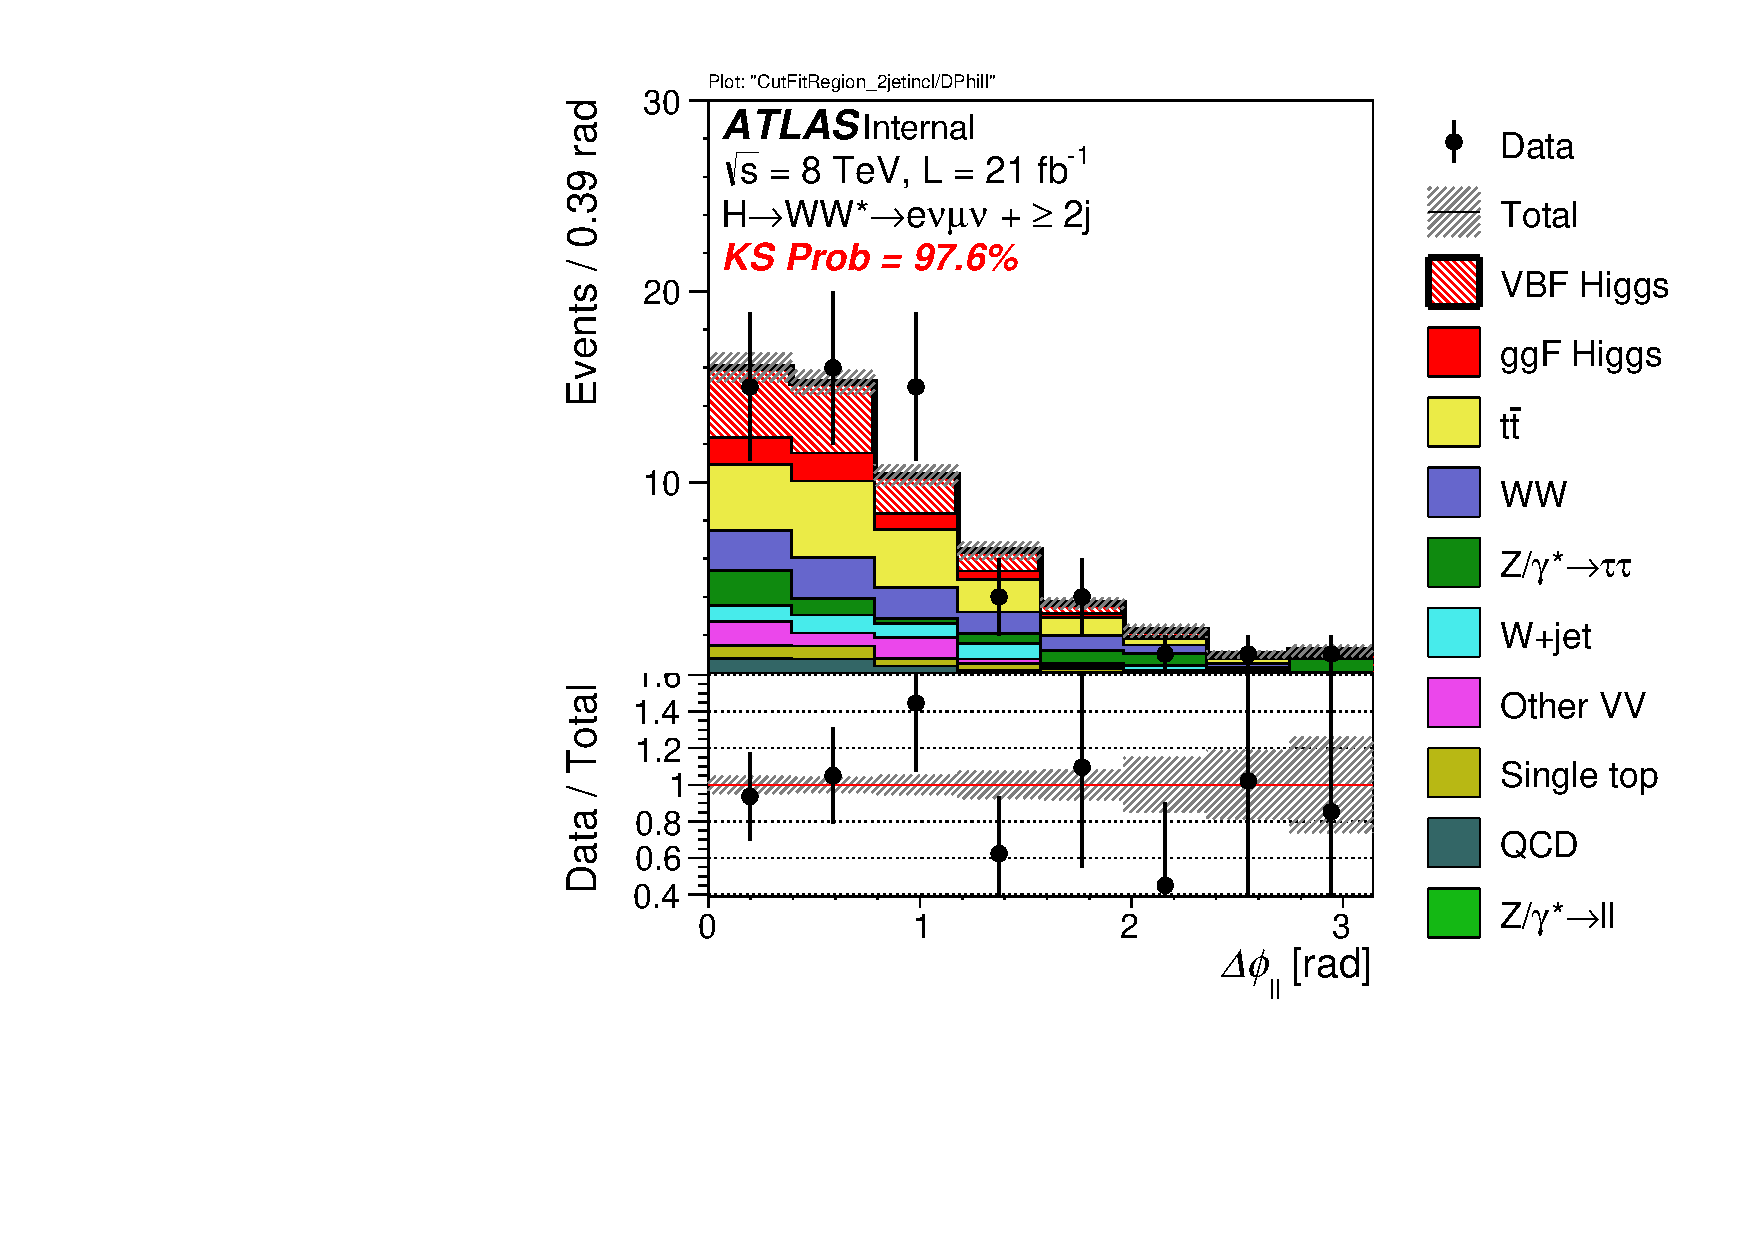
\includegraphics[width=0.4\textwidth]{fig/analysis/BDTinputVarsInSR/DF_SR_FitRegion_DPhill_mh125_lin.pdf}
   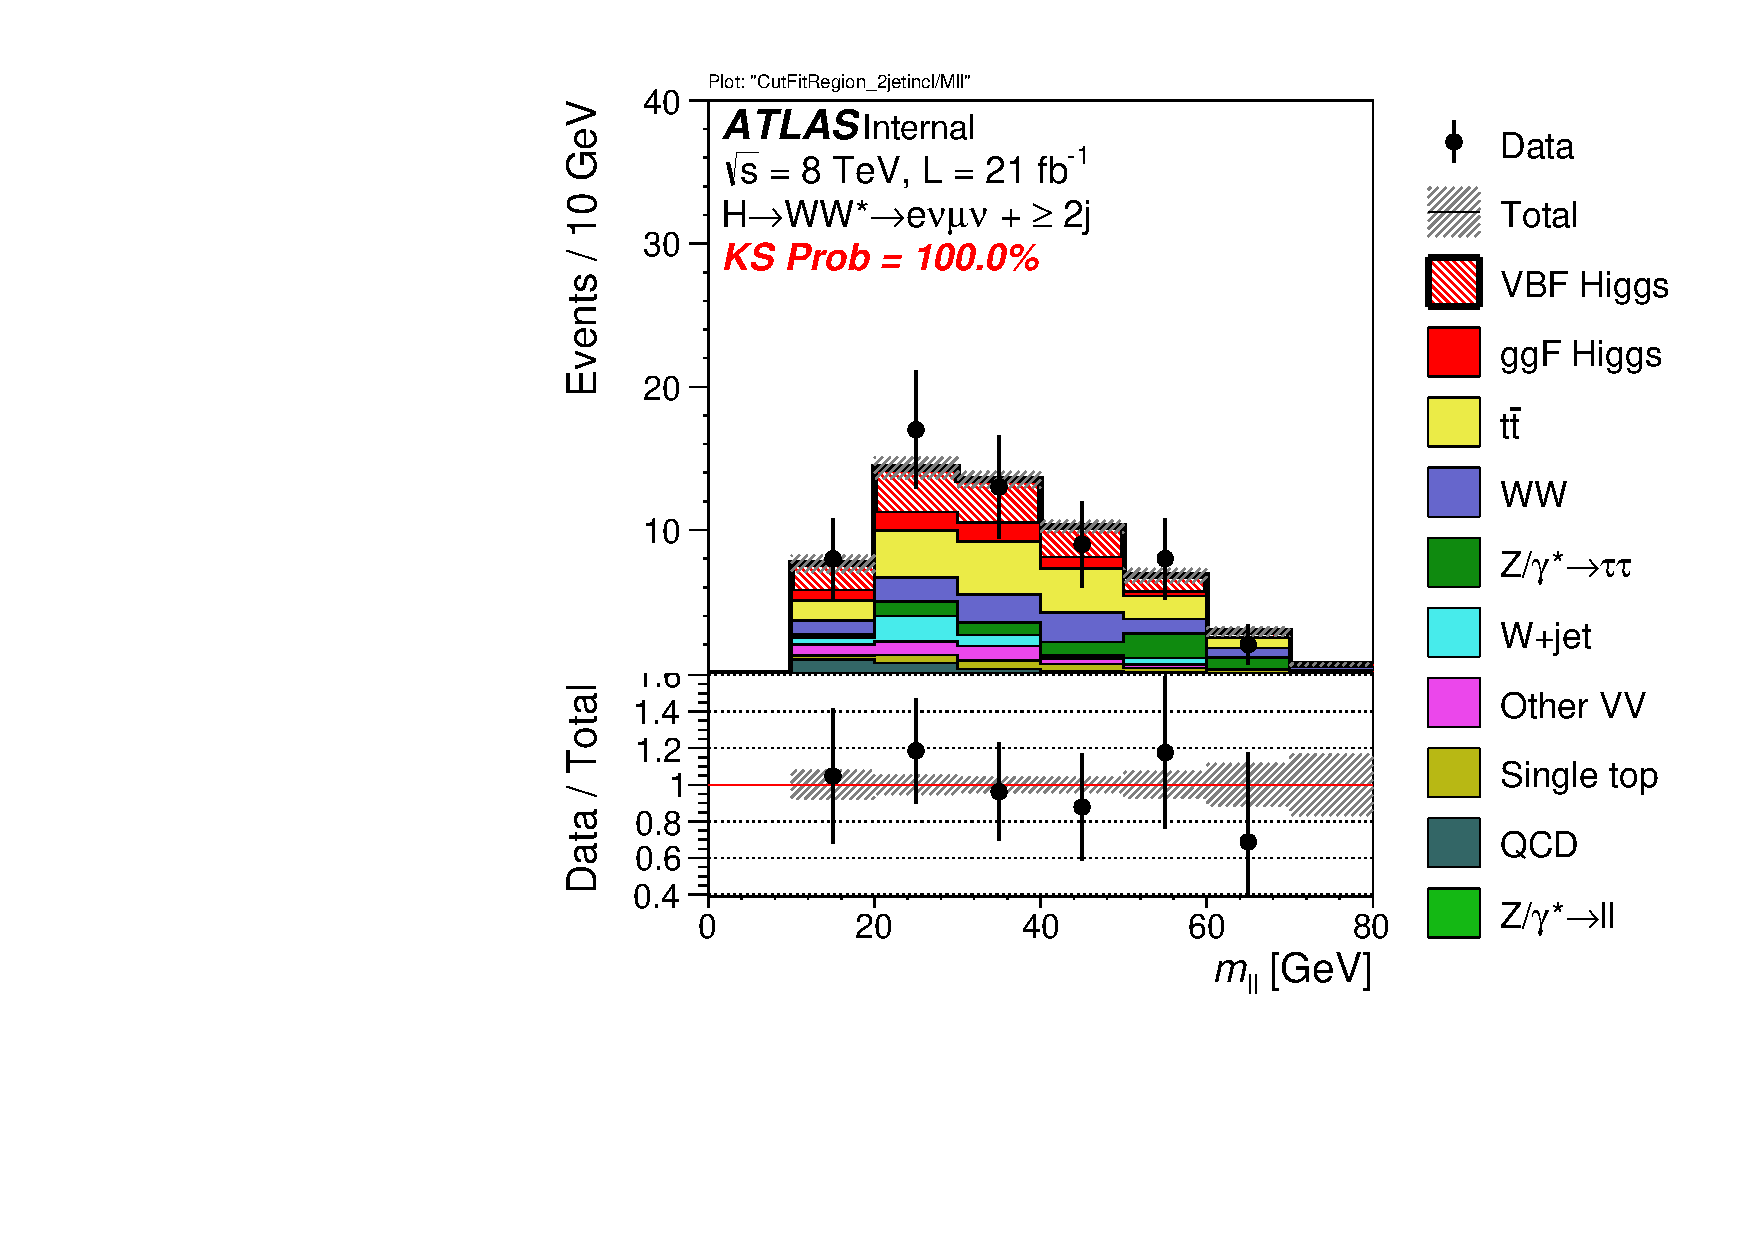
\includegraphics[width=0.4\textwidth]{fig/analysis/BDTinputVarsInSR/DF_SR_FitRegion_Mll_mh125_lin.pdf}
   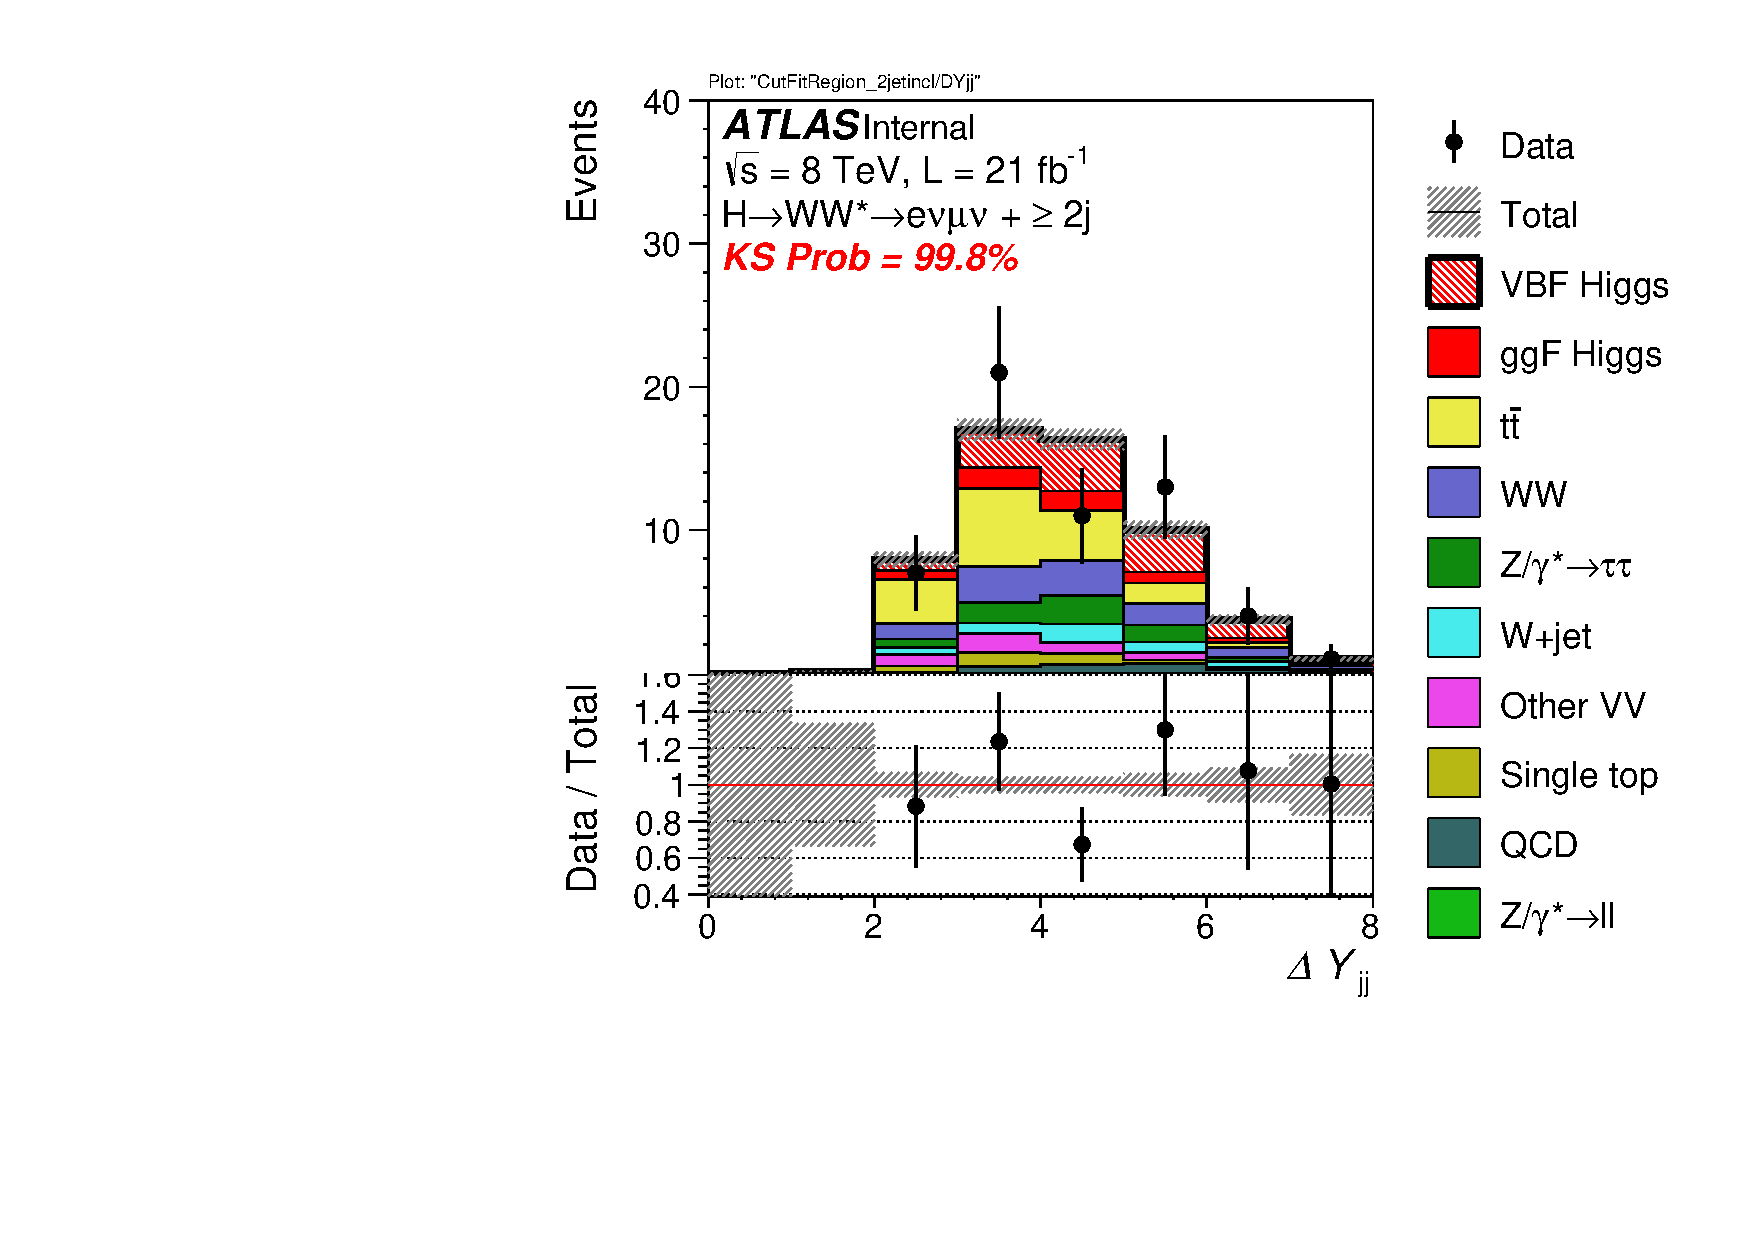
\includegraphics[width=0.4\textwidth]{fig/analysis/BDTinputVarsInSR/DF_SR_FitRegion_DYjj_mh125_lin.pdf}
   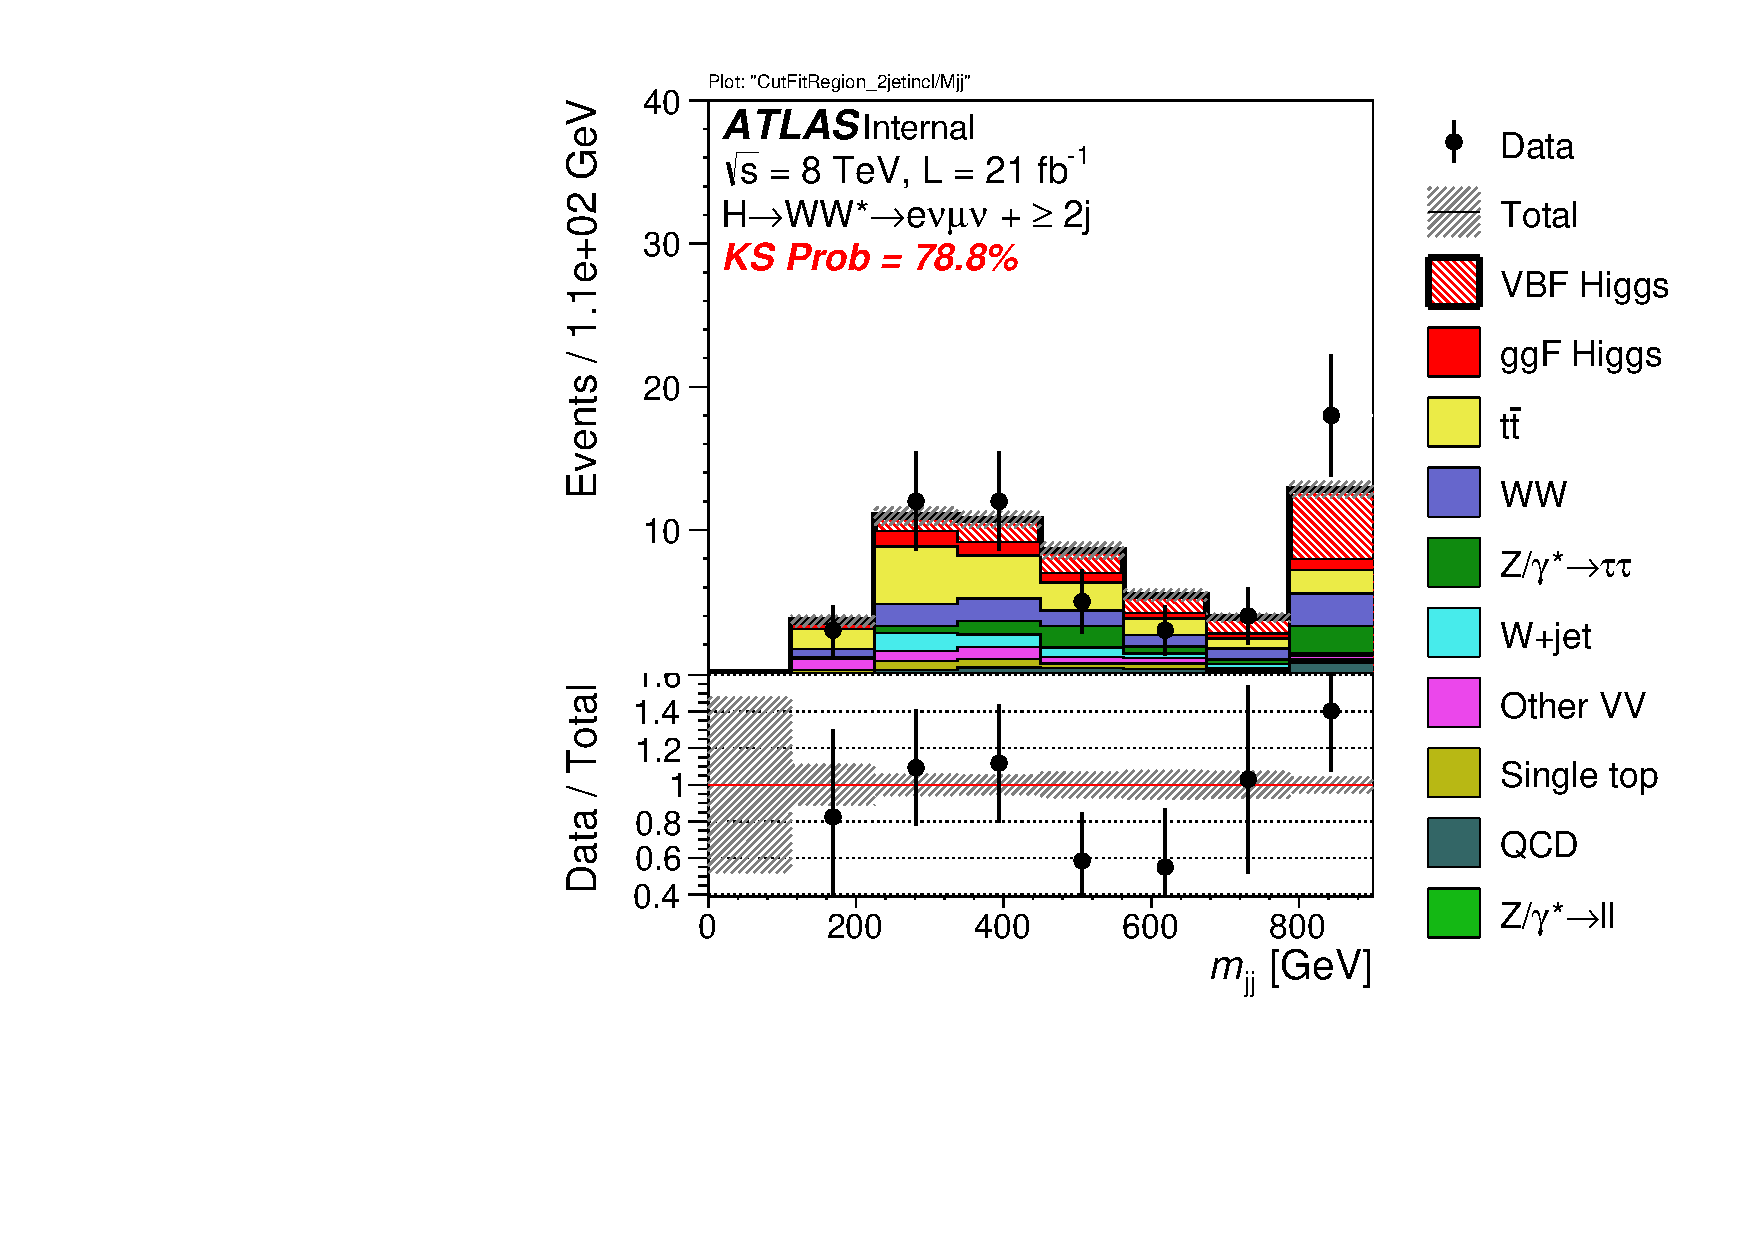
\includegraphics[width=0.4\textwidth]{fig/analysis/BDTinputVarsInSR/DF_SR_FitRegion_Mjj_mh125_lin.pdf}
   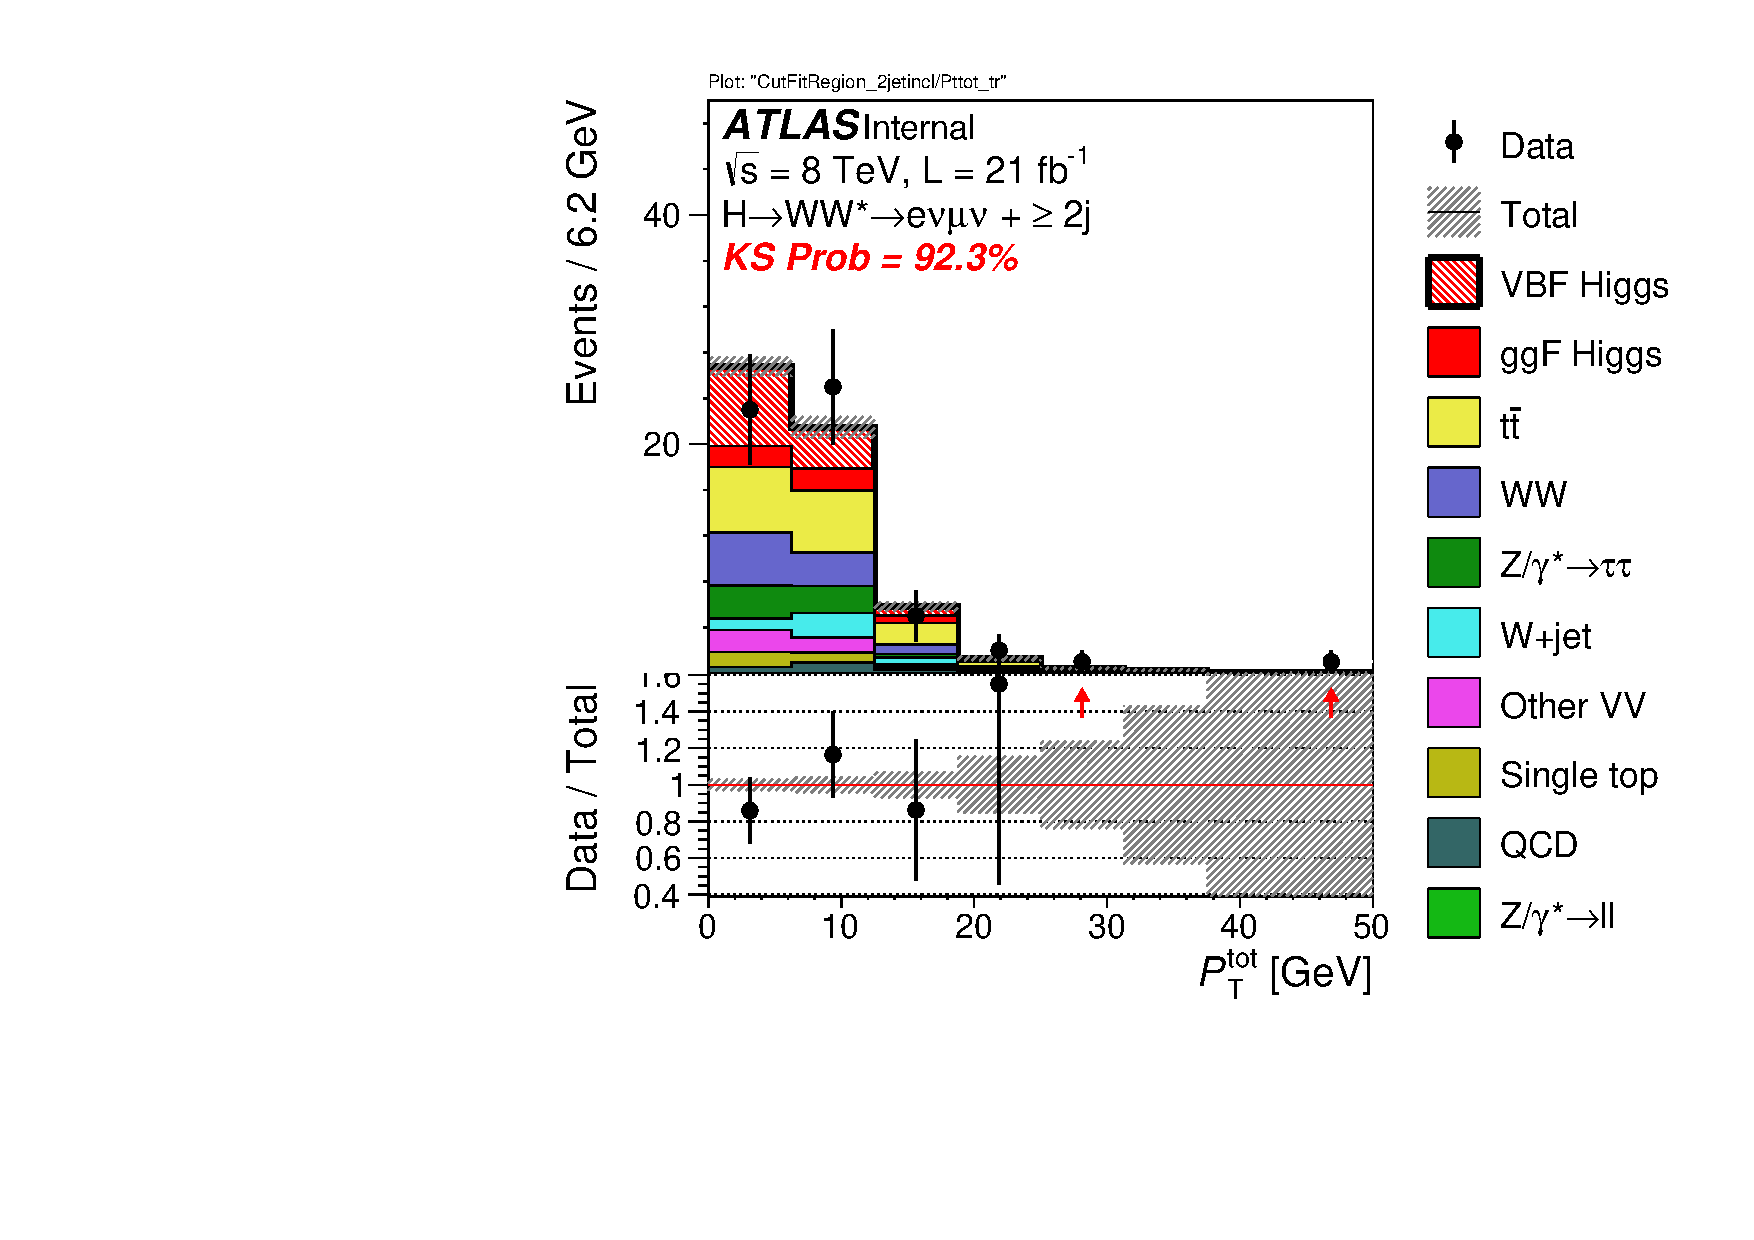
\includegraphics[width=0.4\textwidth]{fig/analysis/BDTinputVarsInSR/DF_SR_FitRegion_Pttot_tr_mh125_lin.pdf}
   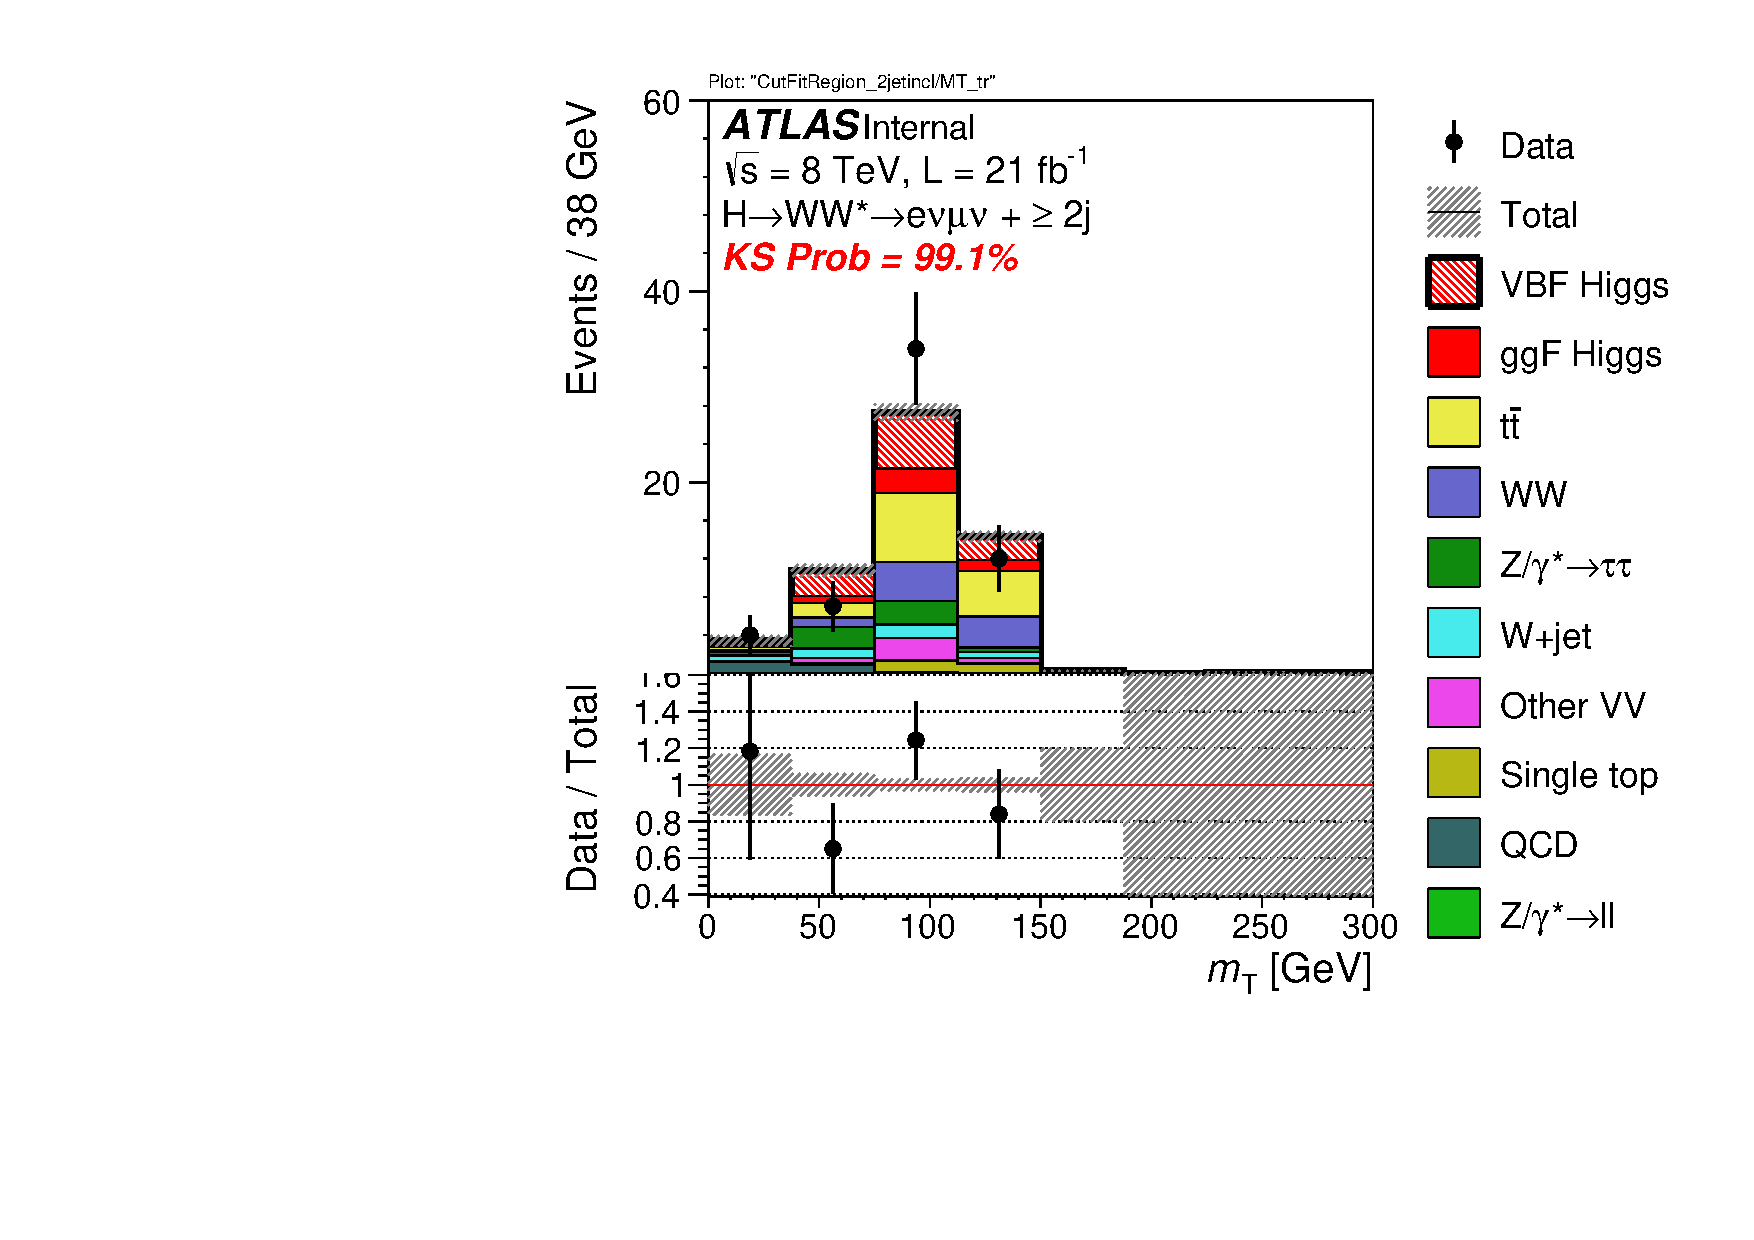
\includegraphics[width=0.4\textwidth]{fig/analysis/BDTinputVarsInSR/DF_SR_FitRegion_MT_tr_mh125_lin.pdf}
   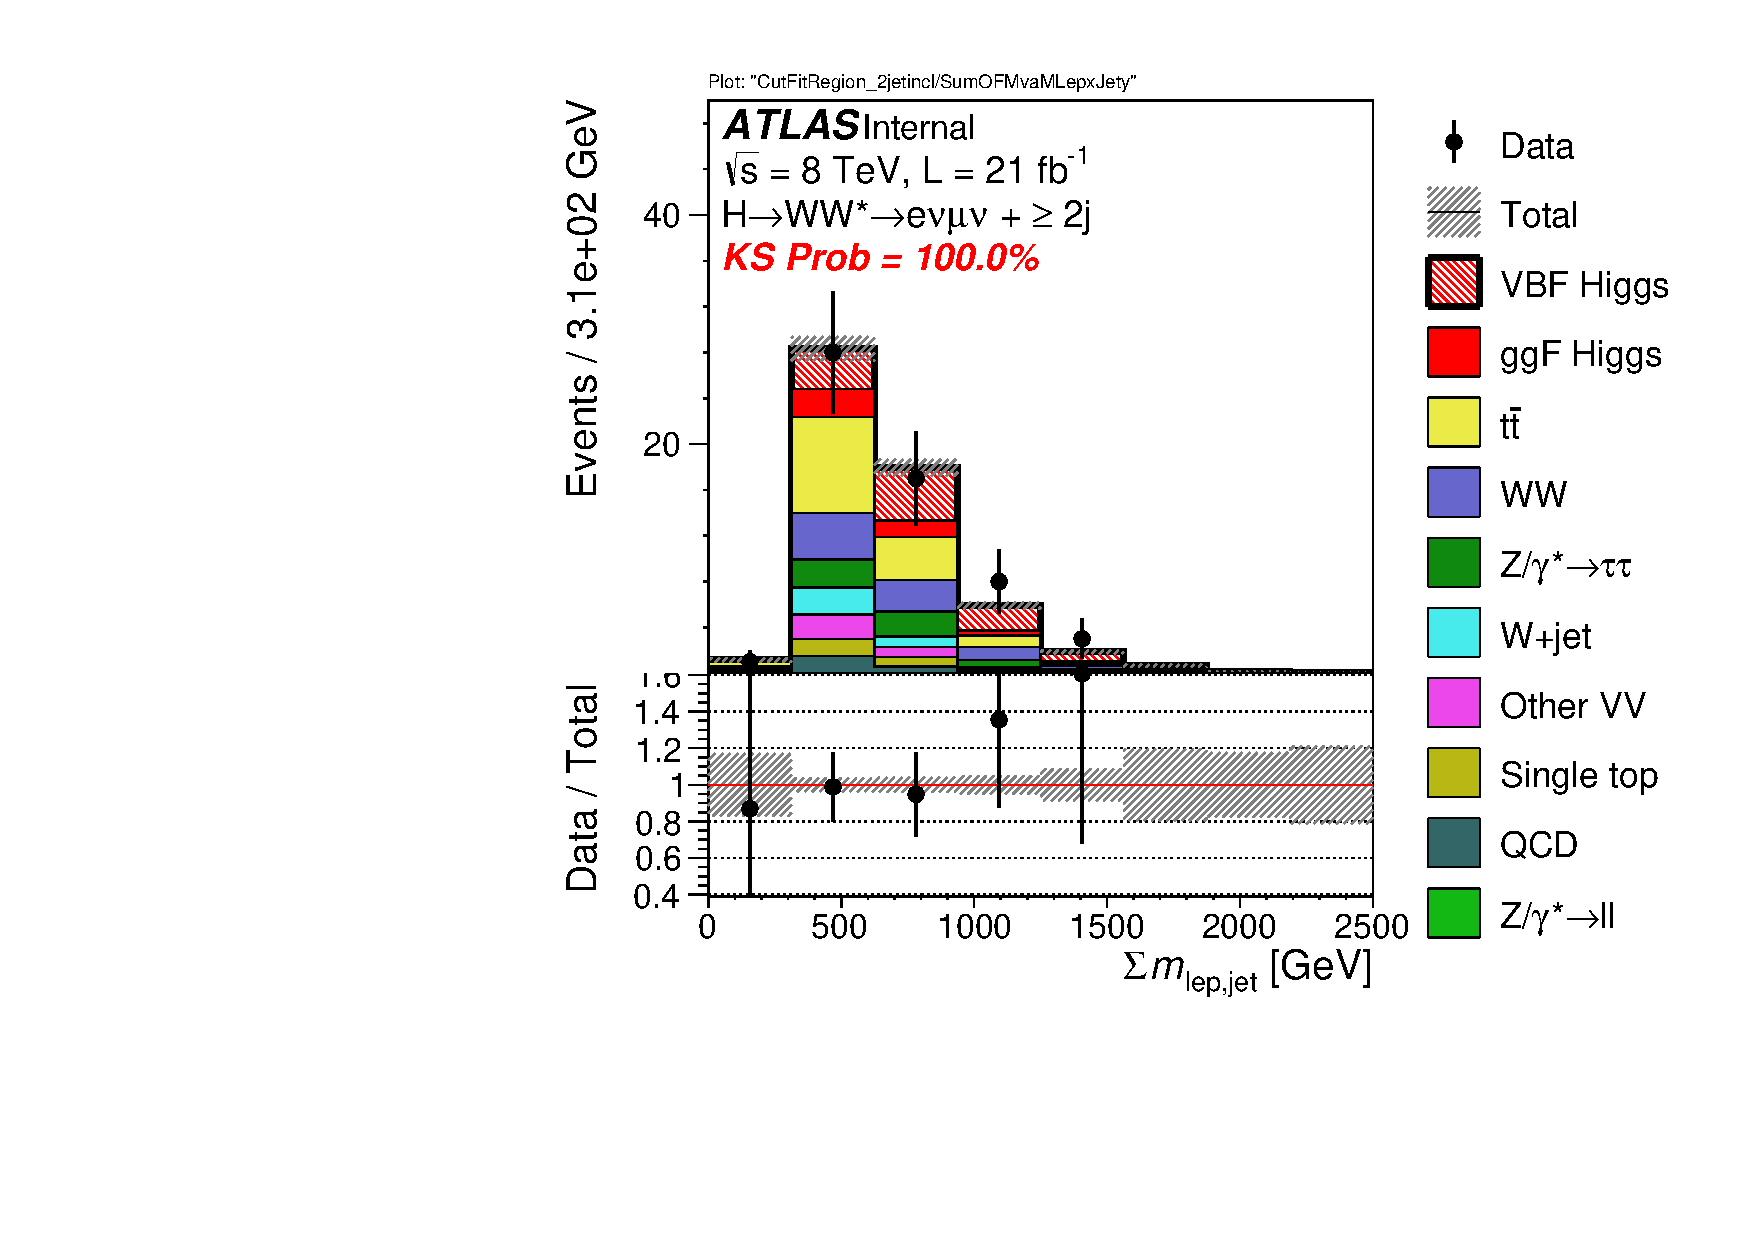
\includegraphics[width=0.4\textwidth]{fig/analysis/BDTinputVarsInSR/DF_SR_FitRegion_SumOFMvaMLepxJety_mh125_lin.pdf}
   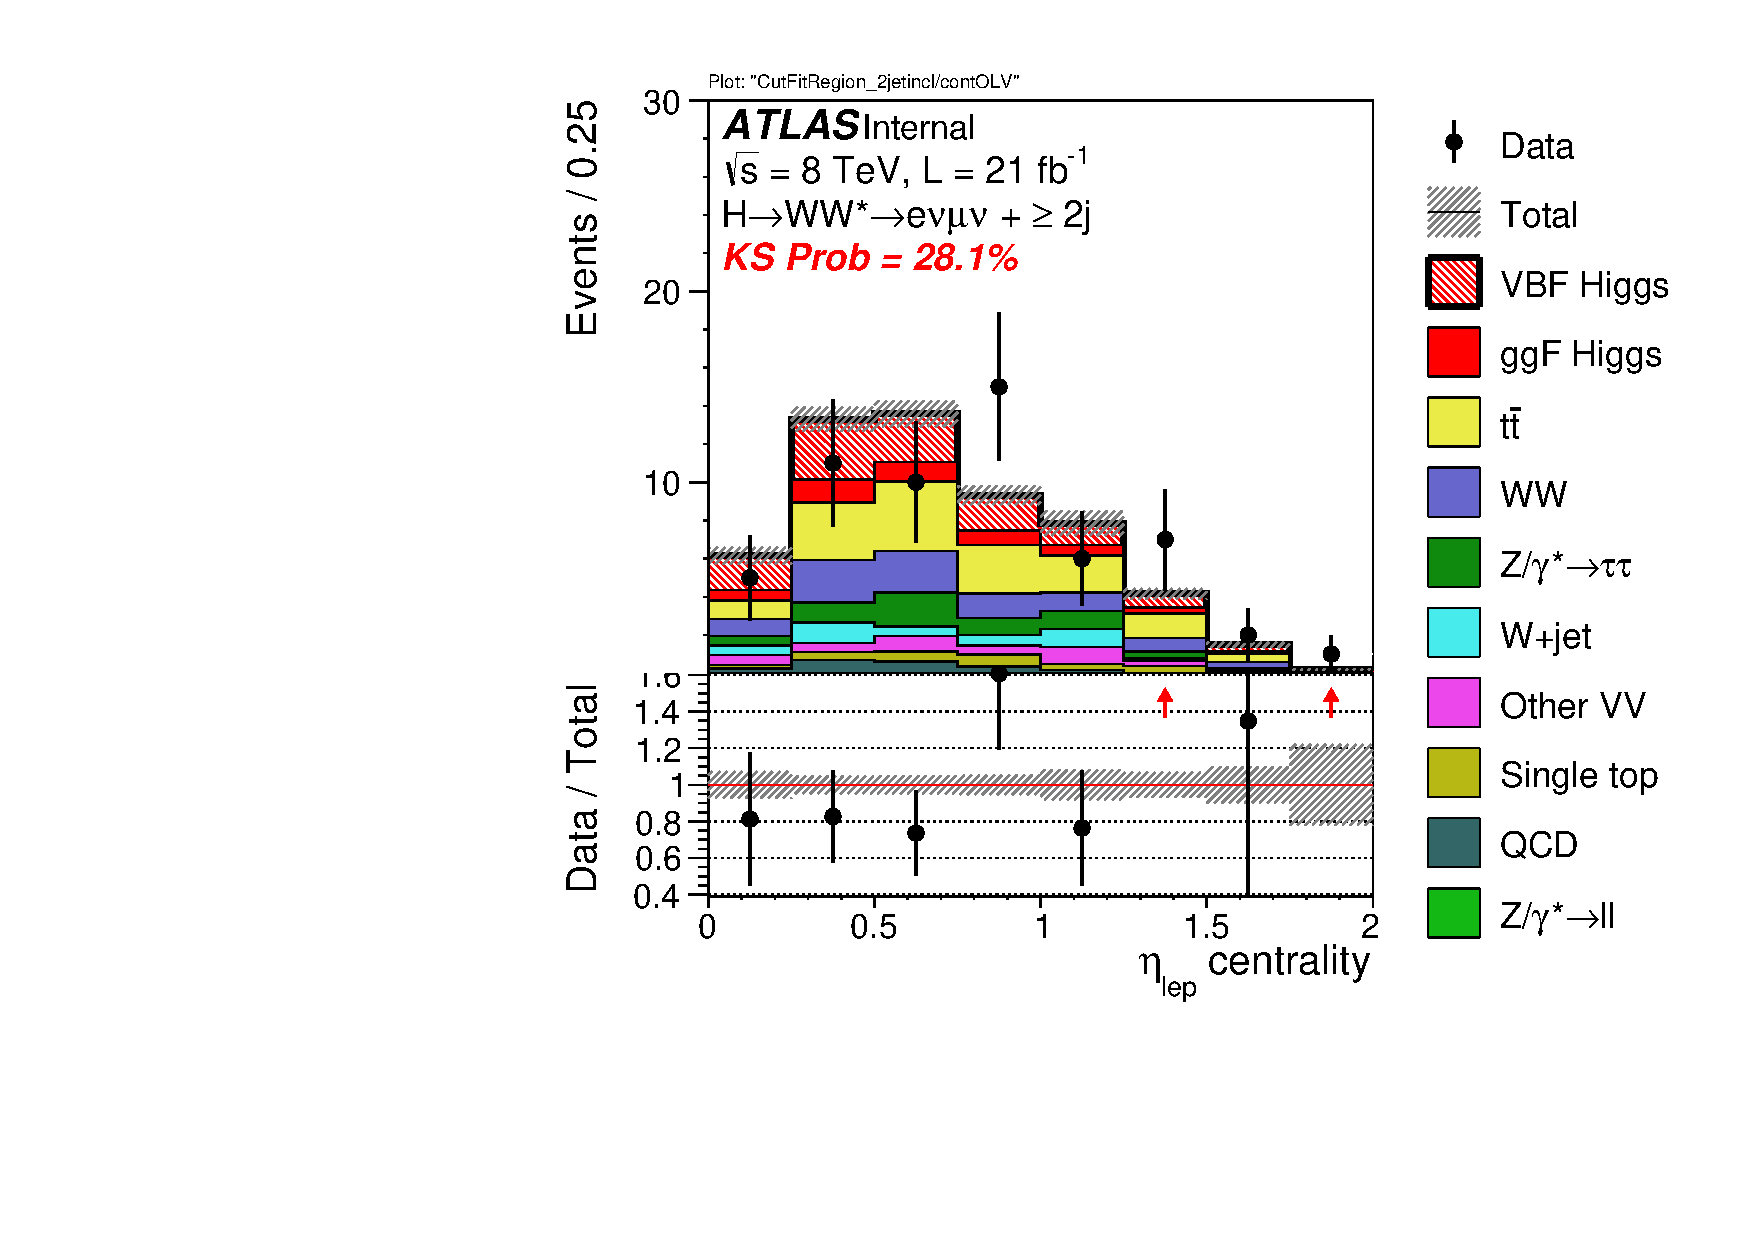
\includegraphics[width=0.4\textwidth]{fig/analysis/BDTinputVarsInSR/DF_SR_FitRegion_contOLV_mh125_lin.pdf}
   \caption{Distributions
   of the eight BDT inputs \dphill, \mll, \dyjj, \mjj, \pTtot, \mT, \SumMlj, and
   \lepEtaCent
   in the \emme channel in the BDT signal region ($\textrm{BDT} > -0.48$).}
  \label{chap:analysis:fig:bdt_inputs_sr_df}
\end{figure}

\begin{figure}[p!]
  \centering
   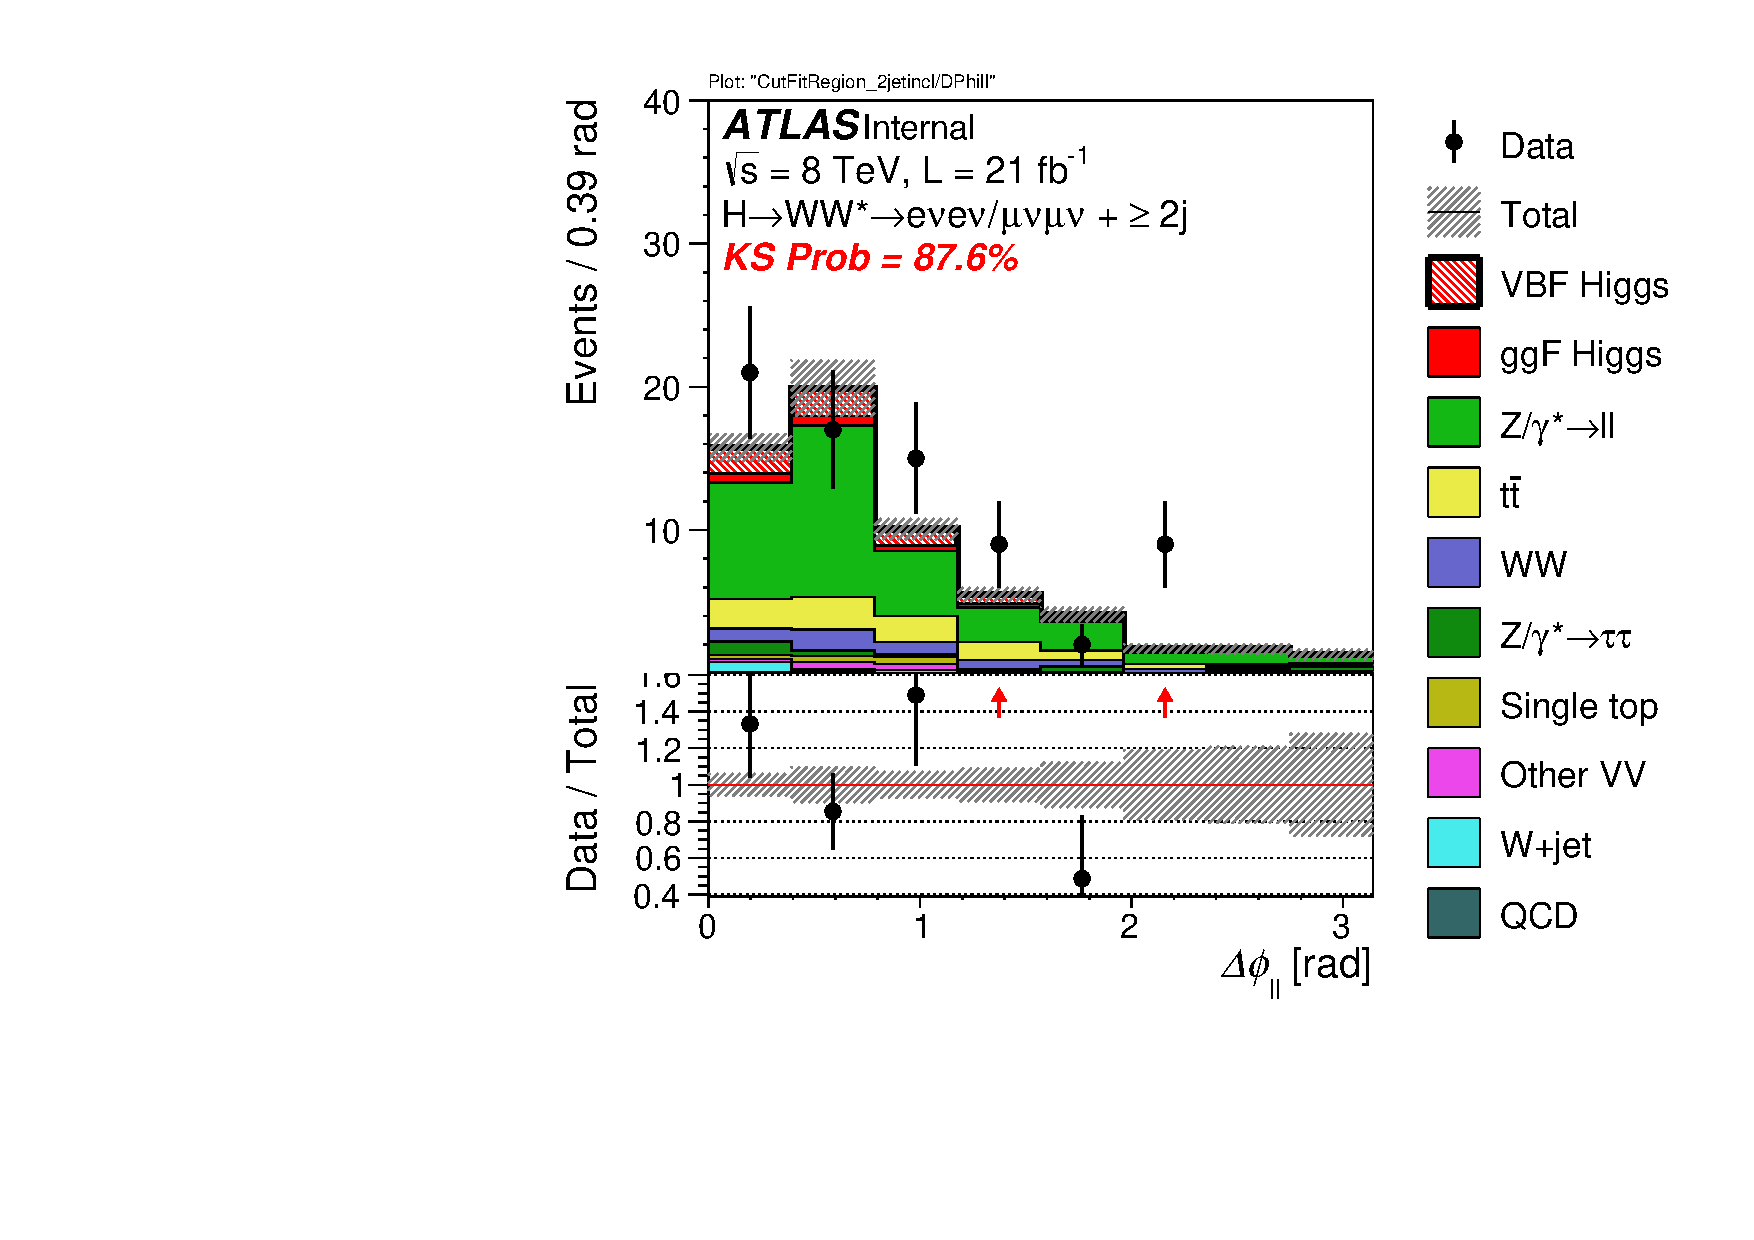
\includegraphics[width=0.4\textwidth]{fig/analysis/BDTinputVarsInSR/SF_SR_FitRegion_DPhill_mh125_lin.pdf}
   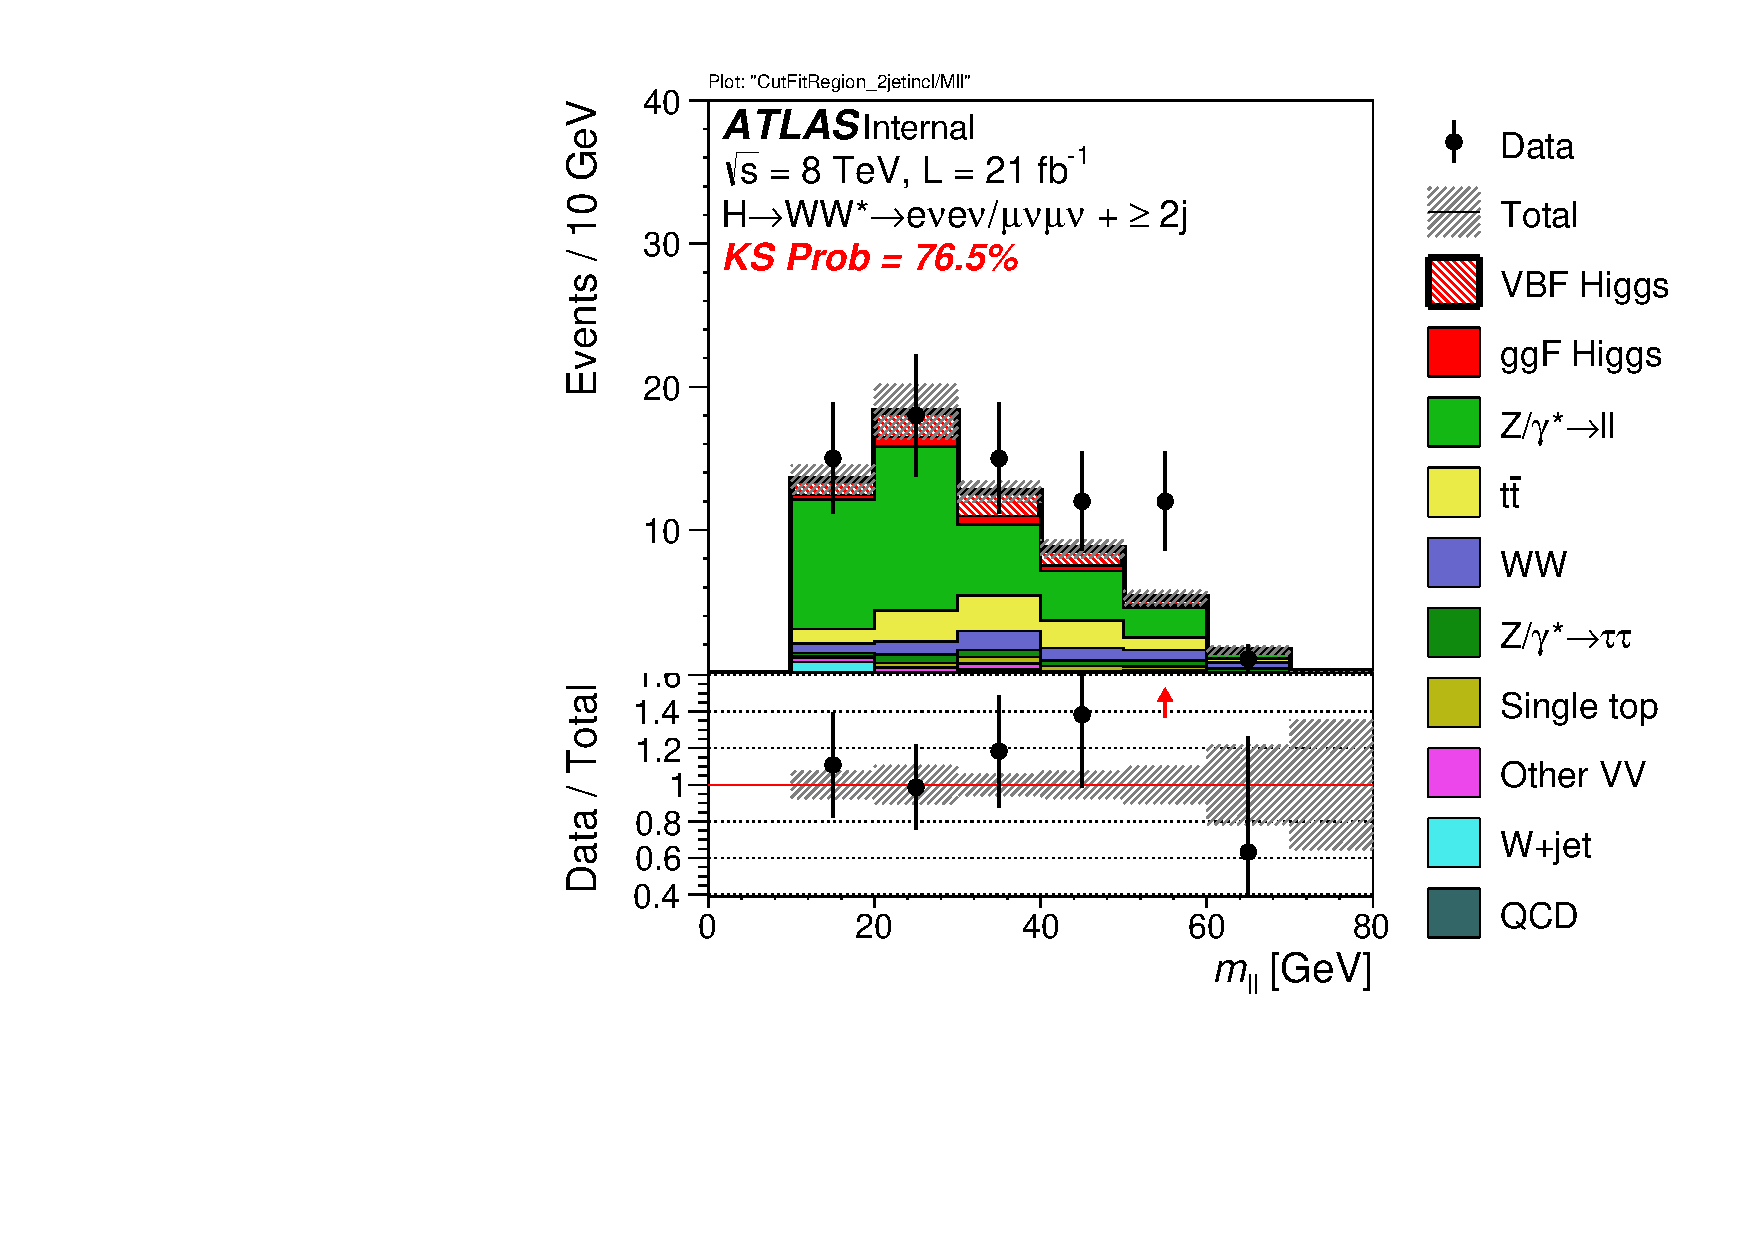
\includegraphics[width=0.4\textwidth]{fig/analysis/BDTinputVarsInSR/SF_SR_FitRegion_Mll_mh125_lin.pdf}
   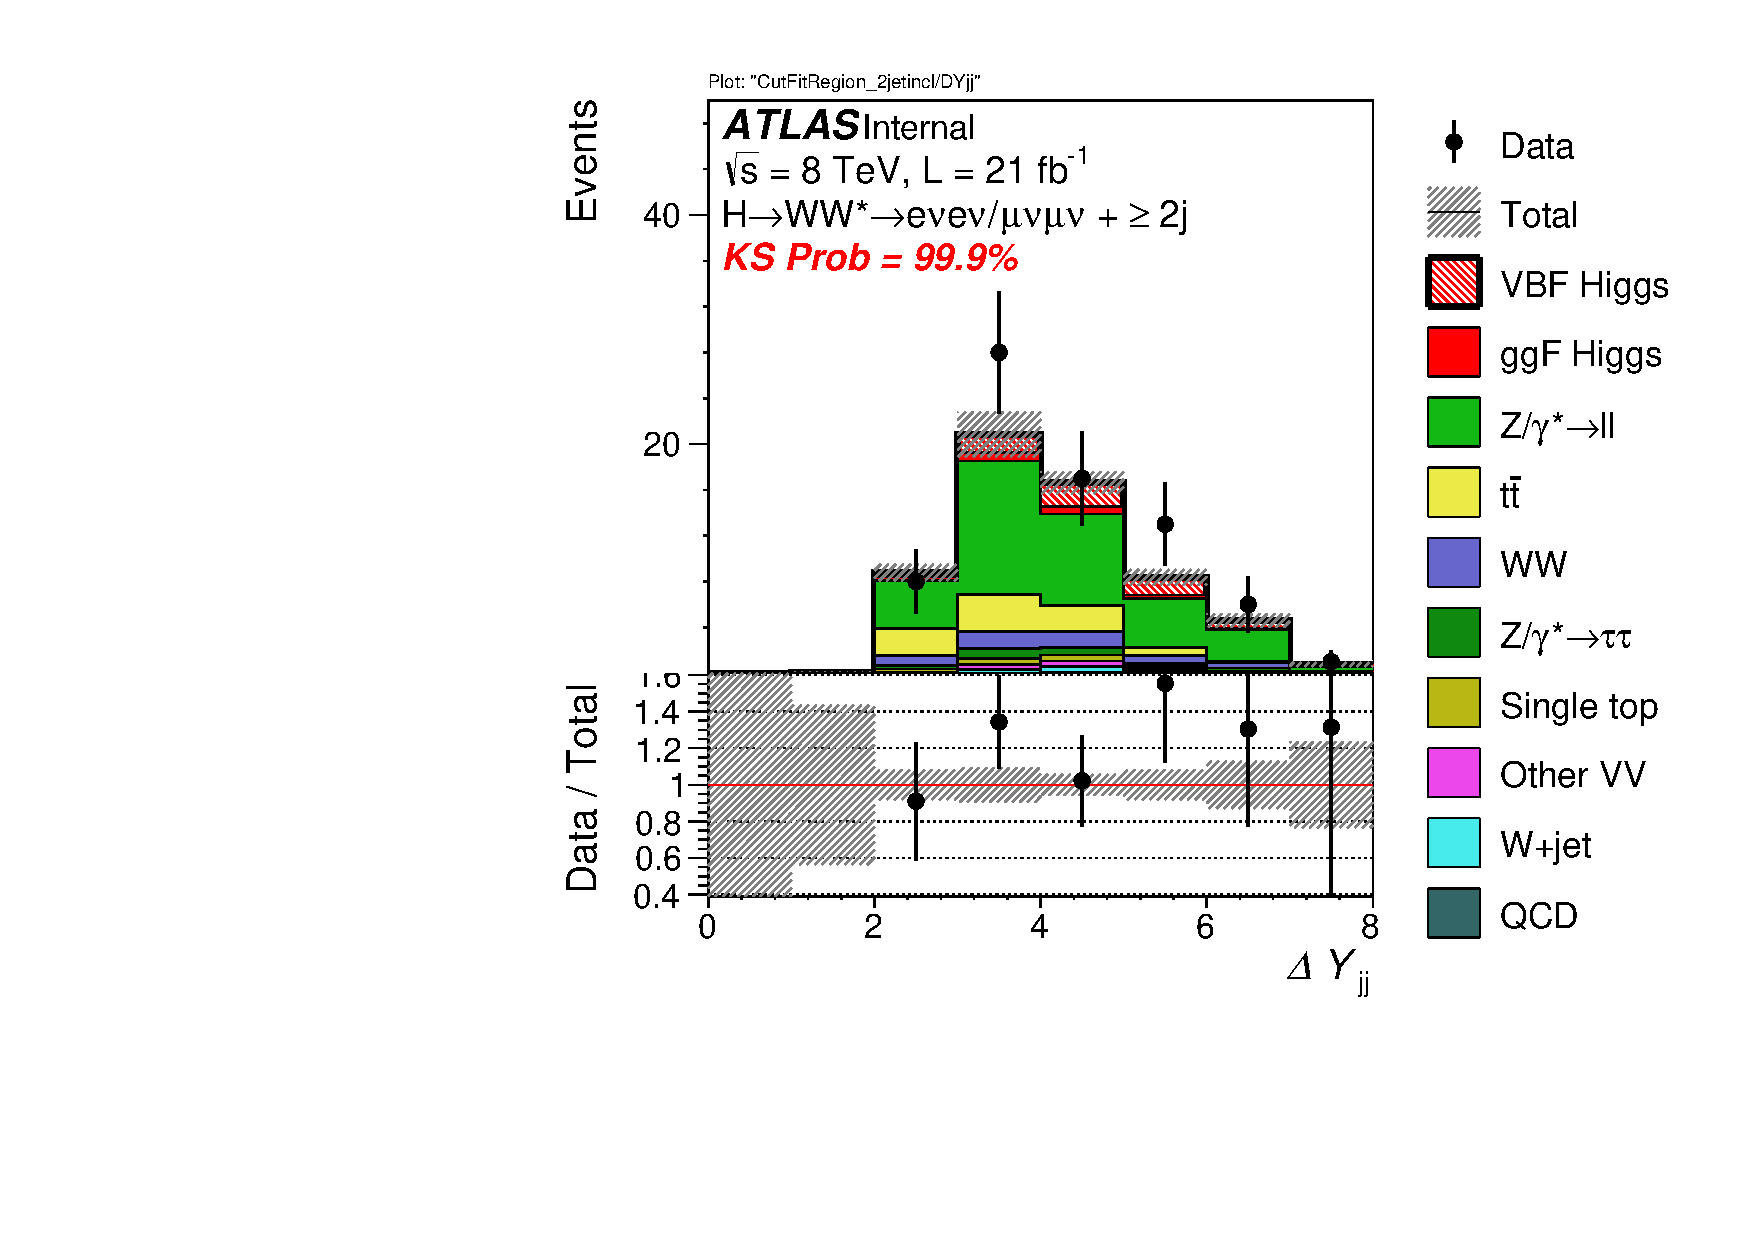
\includegraphics[width=0.4\textwidth]{fig/analysis/BDTinputVarsInSR/SF_SR_FitRegion_DYjj_mh125_lin.pdf}
   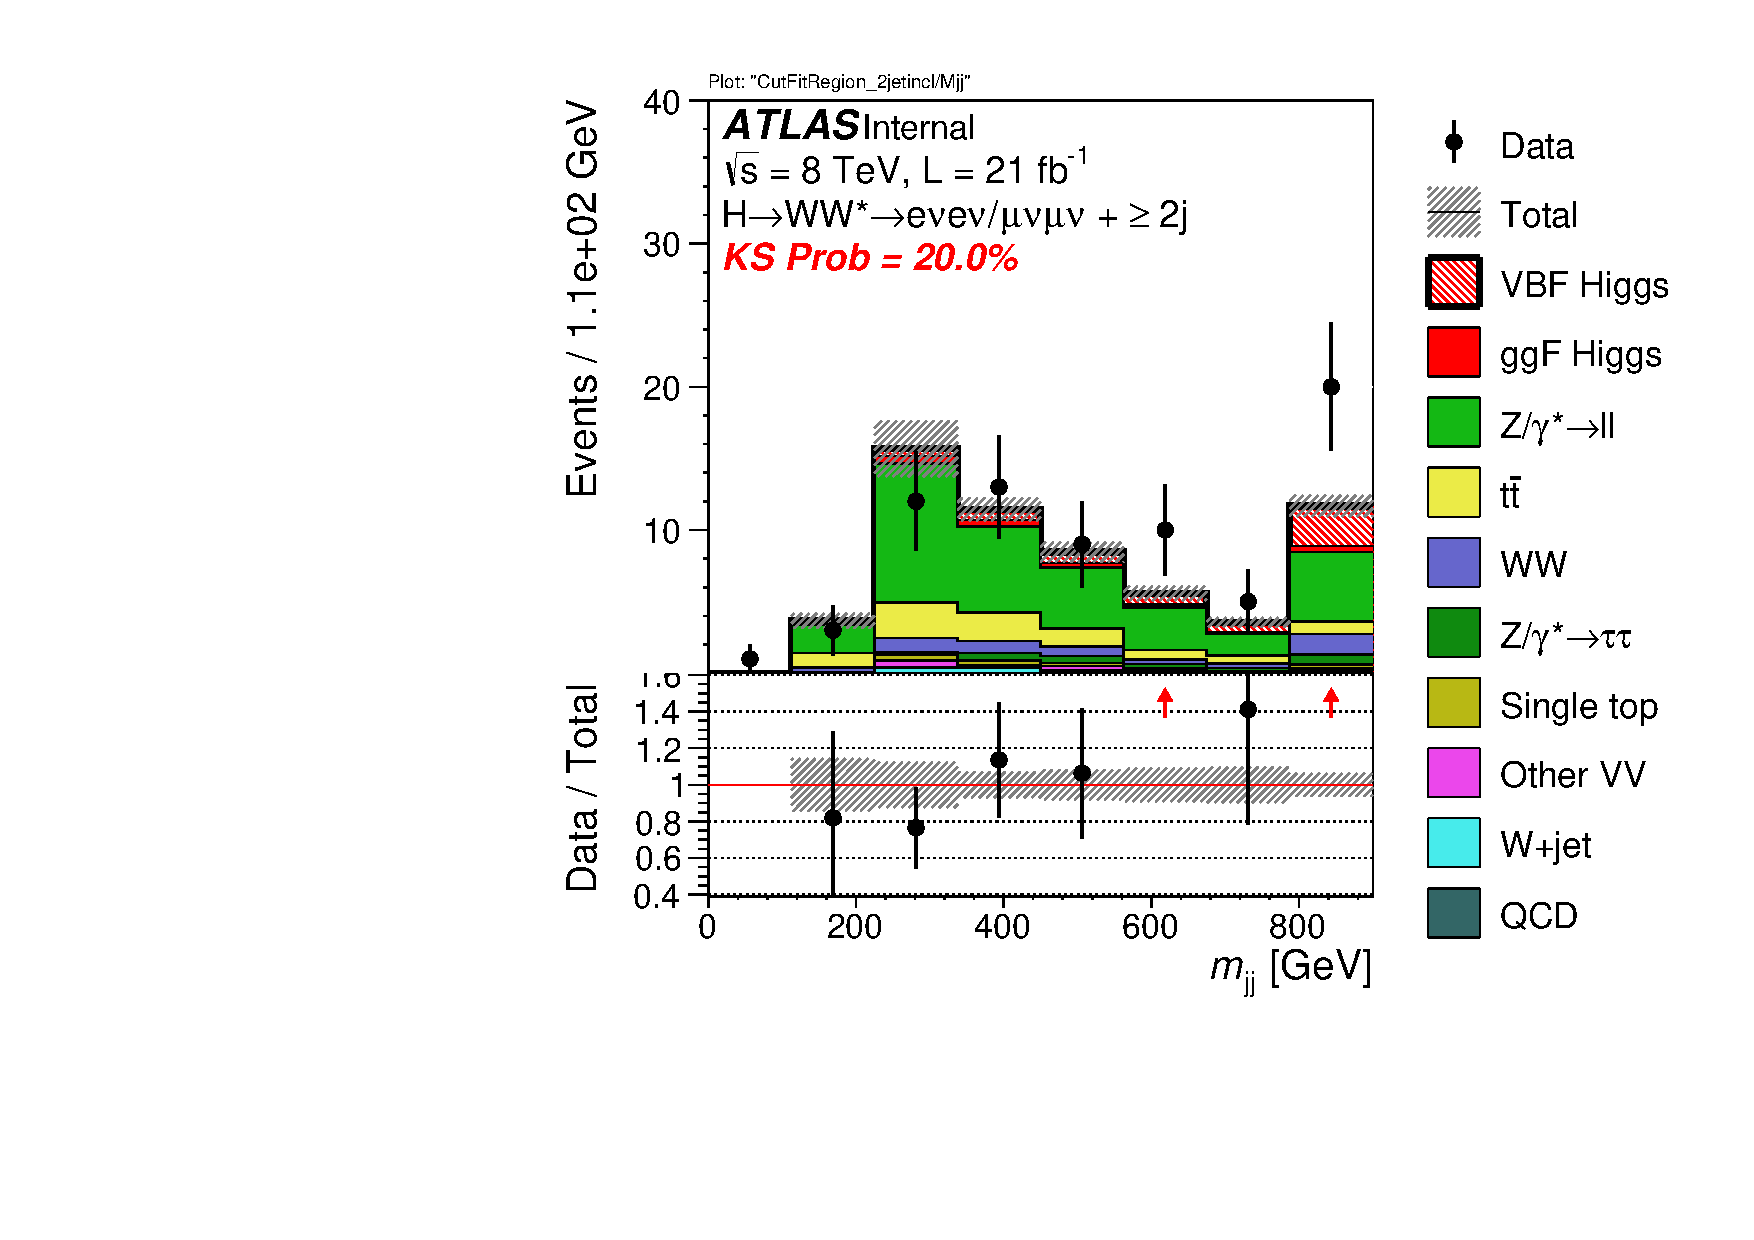
\includegraphics[width=0.4\textwidth]{fig/analysis/BDTinputVarsInSR/SF_SR_FitRegion_Mjj_mh125_lin.pdf}
   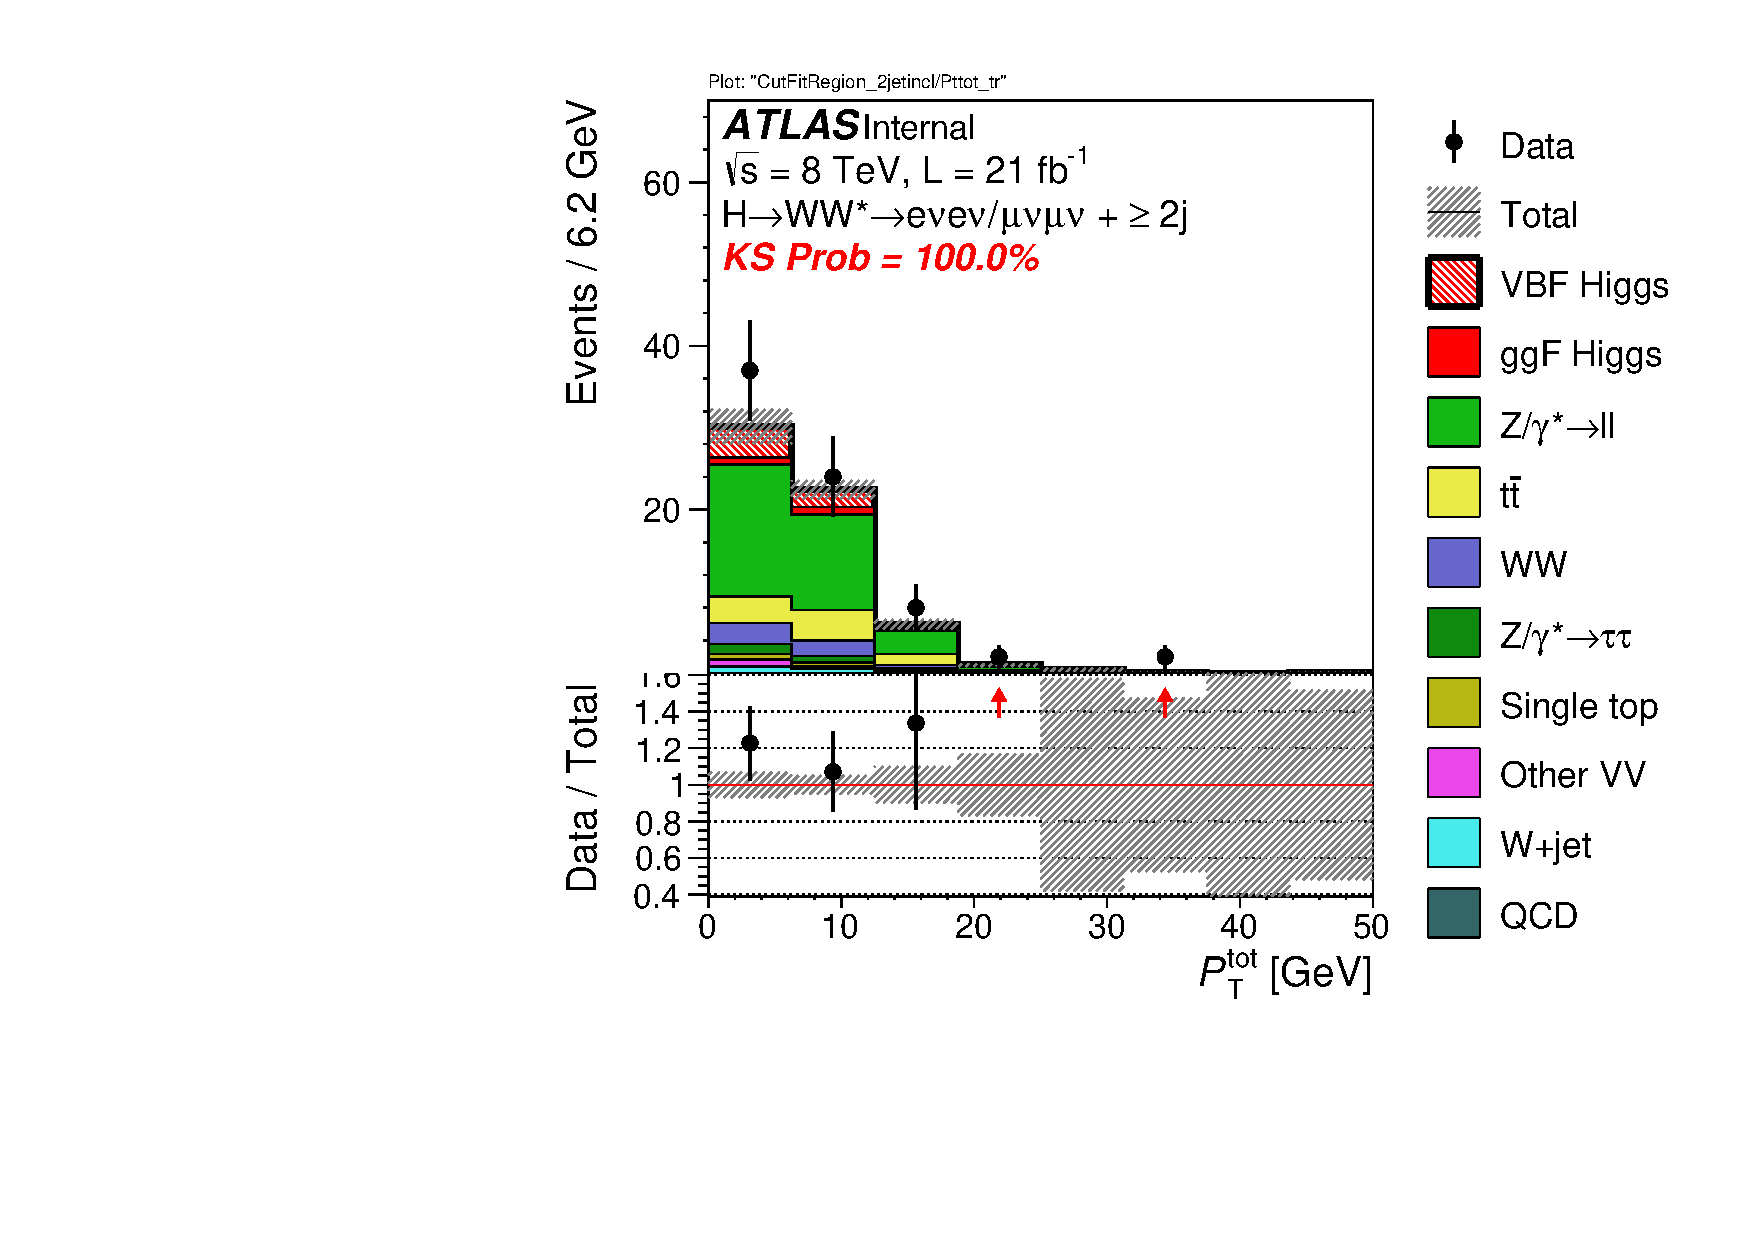
\includegraphics[width=0.4\textwidth]{fig/analysis/BDTinputVarsInSR/SF_SR_FitRegion_Pttot_tr_mh125_lin.pdf}
   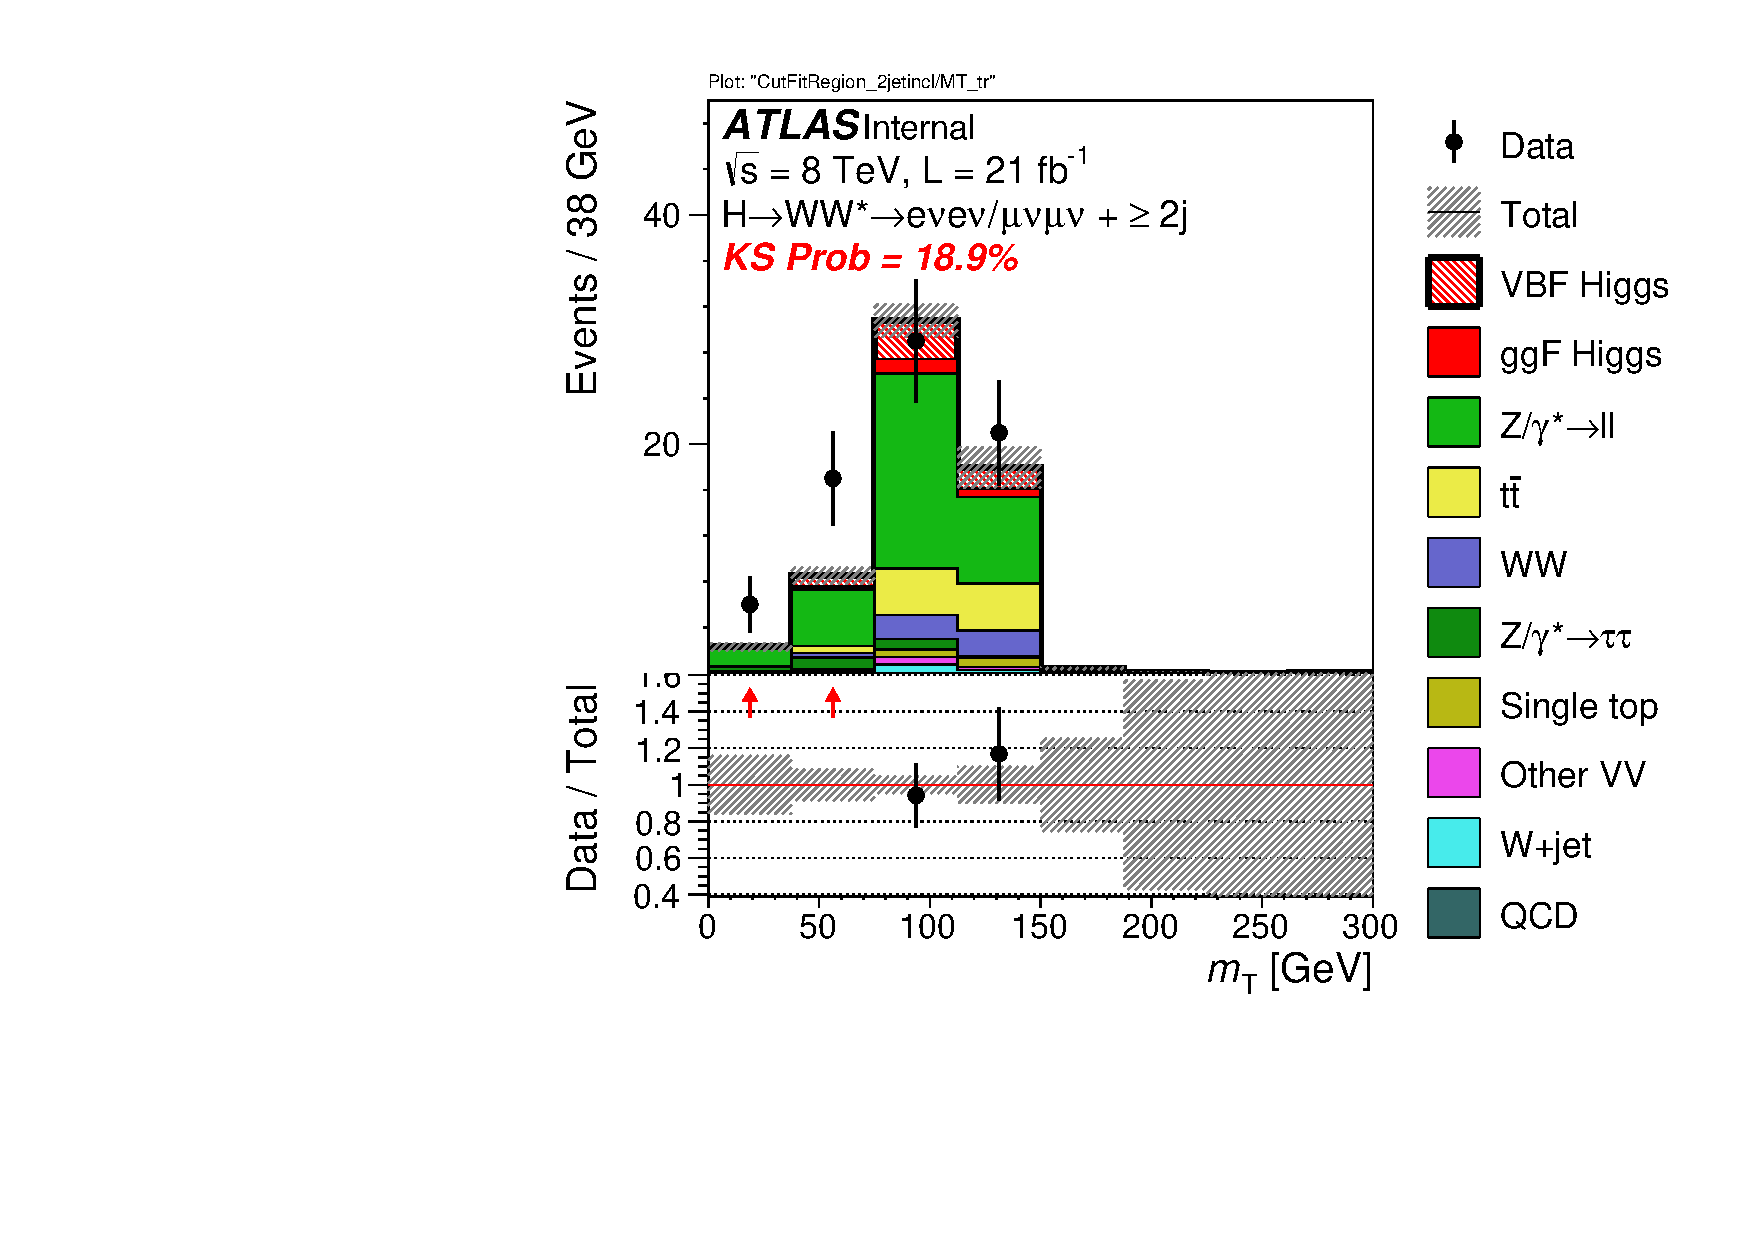
\includegraphics[width=0.4\textwidth]{fig/analysis/BDTinputVarsInSR/SF_SR_FitRegion_MT_tr_mh125_lin.pdf}
   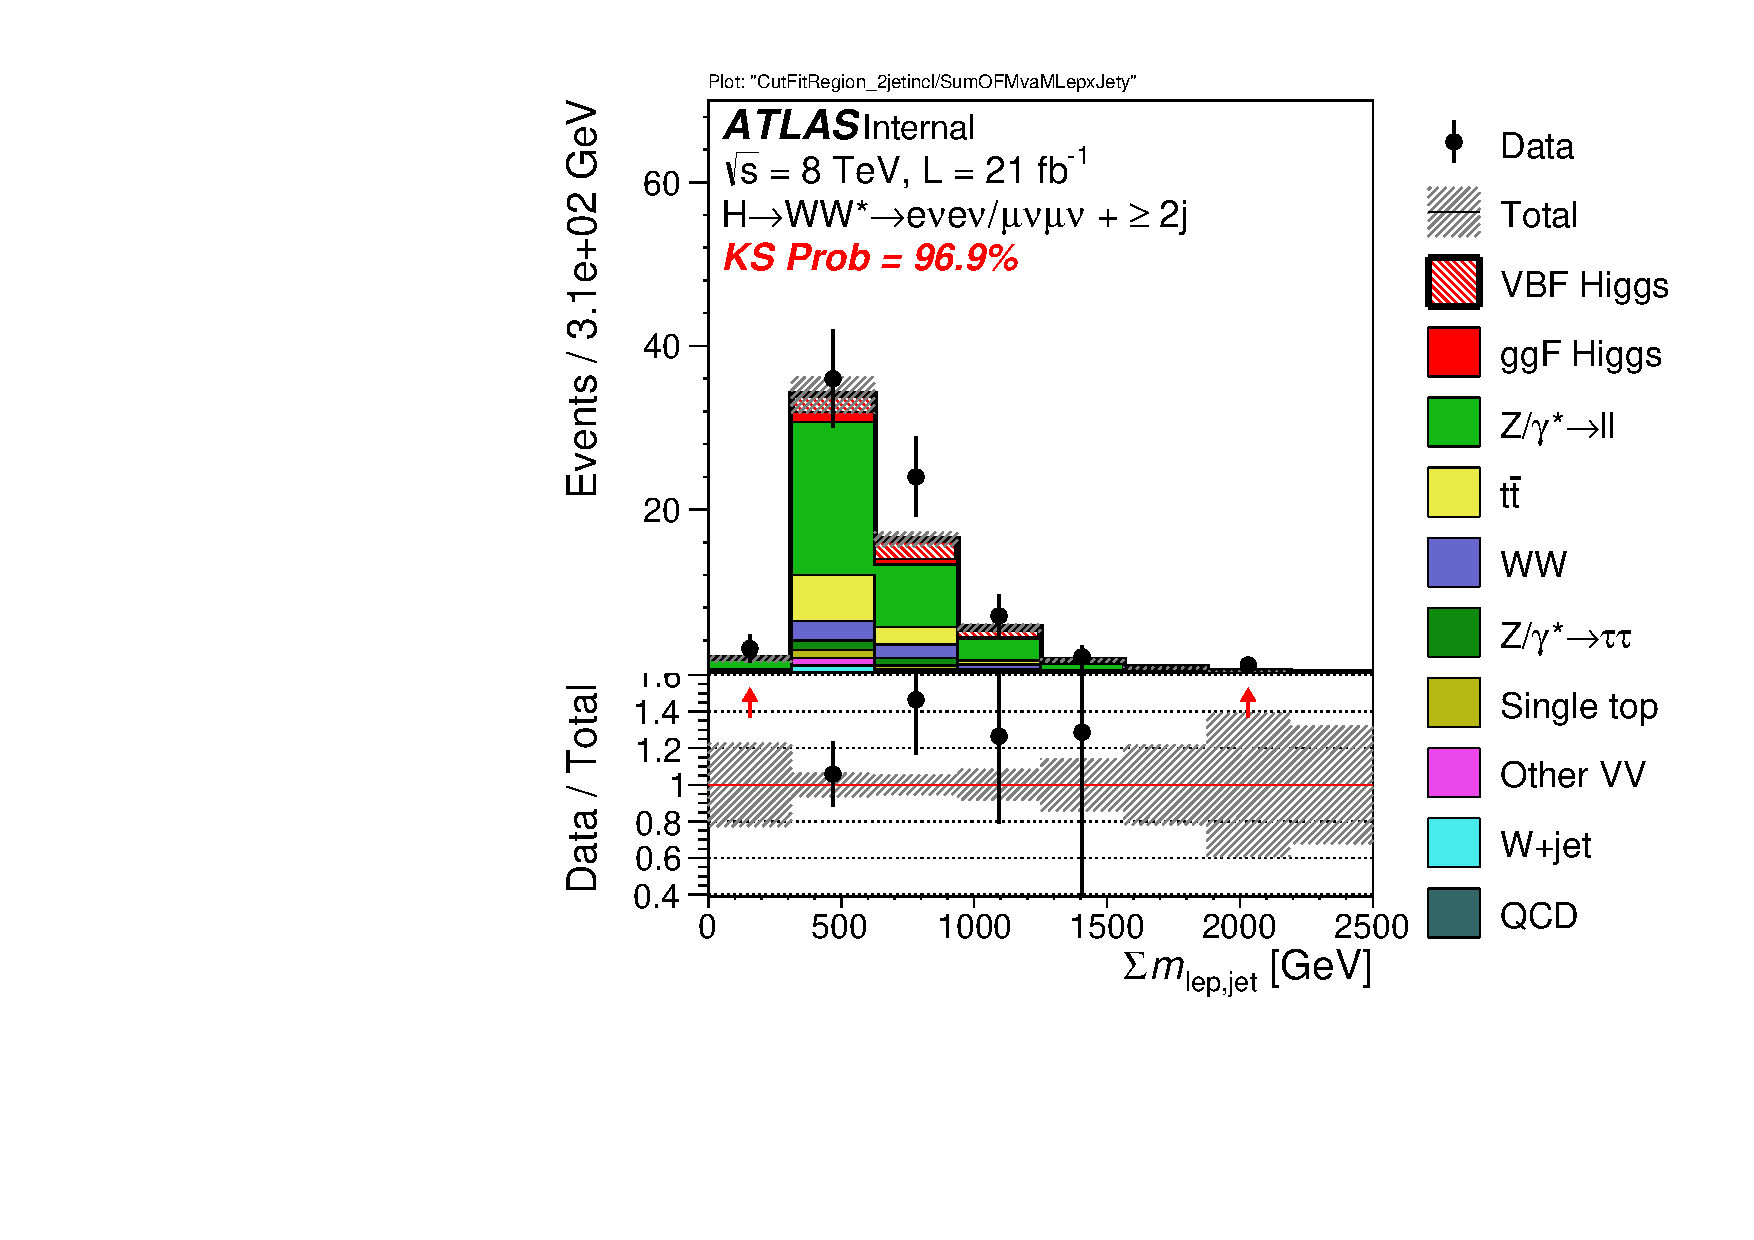
\includegraphics[width=0.4\textwidth]{fig/analysis/BDTinputVarsInSR/SF_SR_FitRegion_SumOFMvaMLepxJety_mh125_lin.pdf}
   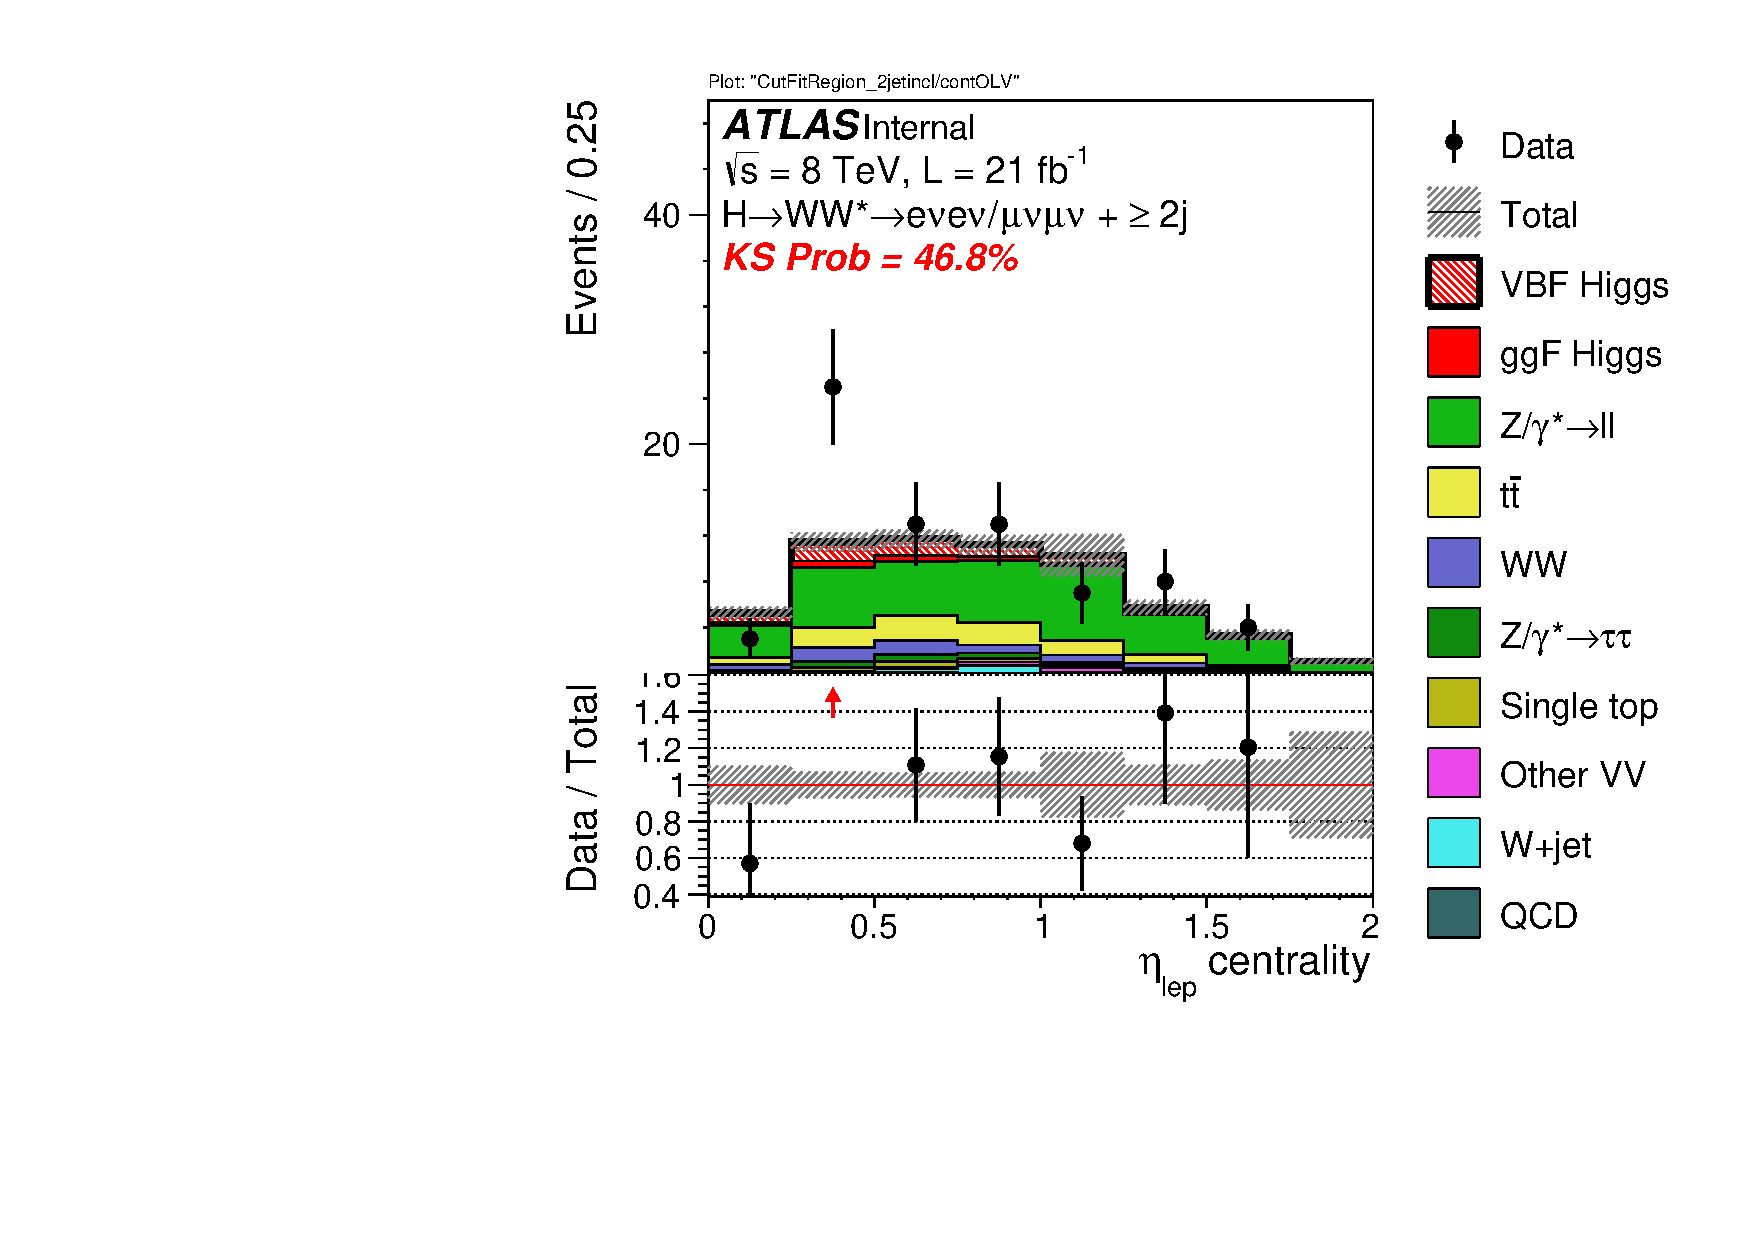
\includegraphics[width=0.4\textwidth]{fig/analysis/BDTinputVarsInSR/SF_SR_FitRegion_contOLV_mh125_lin.pdf}
   \caption{Distributions
   of \dphill, \mll, \dyjj, \mjj, \pTtot, \mT, \SumMlj, and
   \lepEtaCent
   in the \eemm channel in the BDT signal region ($\textrm{BDT} > -0.48$).}
  \label{chap:analysis:fig:bdt_inputs_sr_sf}
\end{figure}


